%

Graph neural networks (GNNs) are a class of ML models which operate on graph representations. Graphs are kind of data structure which describes a set objects (via nodes) and their relationships (via edges). GNNs capture the non-Euclidean arbitrary relational structure of graphs via so-called message-passing/graph-convolutional operations. As a consequence of message-passing operations, GNNs have inbuilt permutation invariance of nodes and edges. An additional useful feature of GNNs is that the same model can deal with graphs with any number of nodes or edges in stark contrast to FFNNs and BDTs which require a fixed input shape and ordering. In the context of event classifiers this allows low-level event objects and their relationships to be encoded on graphs with arbitrary object multiplicity. This analysis utilises a mass-parameterised GNN binary classifier to discriminate signal events against background events. A graph, $G$, which encodes an event and a pseudo mass, $m_H$, are input to the GNN as,

\begin{equation}
    y=\mathrm{GNN}(G, m_H)
\end{equation}

which returns a classification score, $y\in[0,1]$. The target classification scores are 0 for background and 1 for signal. 

\subsubsection{Graph Representation of Events and Input Variables}
In this section the construction of graphs from events will be detailed. The graphs constructed are homogeneous, fully-connected digraphs with no self connections. Within this framework an event graph is defined as a 3-tuple $G=(\textbf{u}, V, E)$ where:

\begin{itemize}
    \item $\textbf{u}$ is a vector of global features representing system level properties of the graph
    \item $V=\{\textbf{v}_i|i\in\{1,...,N\}\}$ is a set of $N$ nodes each carrying a vector, $\textbf{v}_i$, of node features corresponding to node $i$
    \item $E=\{\textbf{e}_{ij}|i\in\{1,...,N\},j\in\{1,...,N\}, i\neq j\}$ is a set of $N(N-1)$ directed edges each carrying a vector, $\textbf{e}_{ij}$, of edge features corresponding to the edge connecting node $i$ to node $j$ 
\end{itemize}
Events are represented on graphs by assigning reconstructed objects and corresponding object-level variables to graph nodes and encoding their respective geometric relationships on edges connecting them. Additionally, event-level variables are included via a set of global graph-level features. The node, edge and global features included on graphs are detailed below:
\begin{itemize}
\item \textbf{Nodes:} The reconstructed objects used to construct nodes include small-$R$ jets, muons, electrons and missing transverse energy. MET is included at node-level rather than as a global features so that the geometric relationship between $\phi_\mathrm{MET}$ and the other reconstructed objects can be encoded on edges. The node features are:
    \begin{itemize}
        \item[--] Object $p_\mathrm{T}$
        \item[--] Object $\eta$ (0 input for MET node)
        \item[--] Object $E$ 
        \item[--] Pseudo-continuous DL1r b-tagging score of the object (0 for non-jets)
        \item[--] Object type encoding number (-2 for muons, -1 for electrons, 0 for MET and 1 for jets)
    \end{itemize}
Object $\phi$ as a node feature is excluded since the $\phi$ geometry of the event is fully captured through the relative $\Delta\phi$ information encoded on directed edges between objects. Removal of absolute $\phi$ values enforces a global $\phi$ symmetry to the graph. A separate scaling factor is applied to each node feature. Fixed scaling factors, $s$, are chosen to map features $x$->$x$/$s$ such that the maximal value of the scaled feature is approximately 1.

\item \textbf{Edges:} Graphs are constructed as fully-connected digraphs by creating an edge for every possible permutation of node pairs. Edge features are calculated from object coordinates in the $(\phi,\eta)$-plane. The edge features are:
    \begin{itemize}
        \item[--] $\Delta \phi$ between pairs of objects
        \item[--] $\Delta \eta$ between pairs of objects
        \item[--] $\Delta R$ between pairs of objects
    \end{itemize}
Separate scaling factors are applied to $\Delta\phi$ and $\Delta\eta$. $\Delta R$ is scaled by the sum of these scaling factors. Fixed scaling factors, $s$, are chosen to map features $x$->$x$/$s$ such that the maximal value of the scaled feature is approximately 1.


\item \textbf{Globals:} The event-level features included in the global variable set include simple bulk properties of the event such as $N_\mathrm{jets}$ and $H_T$ but also high-level reconstructed variables which have been shown to provide discriminating power. The set of variables is adapted from the BDT input set detailed in section \ref{sec:BDT-input-variables} by removing features otherwise included via nodes e.g leading jet $p_\mathrm{T}$ and MET. The global features are:
    \begin{itemize}
        \item[--] $H_T=\sum_i \pT^i$ where the sum is over all reconstructed jets and leptons
        \item[--] The $H_T$ of the first 4 leading jets ranked in order of descending \pt divided by the $H_T$ of the remaining jets, $\sum_{i<4}\pt^i/\sum_{i\geq4}\pt^i$
        \item[--] Average invariant mass of jets triplets with separation $\Delta R<3$
        \item[--] For the 2L channel only: Invariant mass of the dilepton pair  $m_{ll}$
        \item[--] For the 1L channel only: $W^\pm$ reconstructed transverse mass $m_T(l,E_\mathrm{T}^\mathrm{miss})$
        \item[--] Jet multiplicity $N_\mathrm{jets}$
        \item[--] Number of RC-jets with mass greater than 100 GeV
        \item[--] Average invariant mass of b-tagged jet triplets
        \item[--] Minimum $\Delta R$ among pairs of b-tagged jet and lepton
        \item[--] Minimum $\Delta R$ among pairs of b-tagged jets
        \item[--] Centrality $\sum_i \pt^i/\sum_i E_i$ where the sums are performed over all reconstructed jets and leptons
        \item[--] Average $\Delta R$ across all jet pairs
        \item[--] Sum of pseudo-continuous b-tagging scores, $\sum_{i<6}pcb_i$, of the first 6 jets ranked in order of descending DL1r scores
        \item[--] Sum of the first $k_t$ splitting scale $d_{12}$ over all RC-jets
        \item[--] Sum of the second $k_t$ splitting scale $d_{23}$ over all RC-jets
    \end{itemize}

\end{itemize}


\subsubsection{A Parameterised General Message Passing GNN}

In this section the inner workings of the message-passing layers developed and the construction of the GNN used in this analysis will be discussed. The GNN used in this analysis is built using the \texttt{PyTorch Geometric} package. In particlular, the \texttt{MetaLayer(torch.nn.Module)} class is utilised which provides a generic building block for creating general GNNs inspired by the framework established in \cite{https://doi.org/10.48550/arxiv.1806.01261}. Within this framework a GNN layer can be split into three models: an edge updating model, a node updating model and a global updating model. Upon application the \texttt{MetaLayer} updates the input graph by applying the edge update followed by the node update followed by the global update. The edge, node and global models are classes which can be explicitly programmed using \texttt{PyTorch}. In this section the forward pass mechanisms of each model will be defined.

\begin{itemize}
    \item \textbf{Edge updating model:} An edge connecting nodes $i$ to node $j$ is updated via
    \begin{equation}
        \textbf{e}_{ij}'=f_\mathrm{edge}(\textbf{v}_i,\textbf{v}_j,\textbf{e}_{ij}, \textbf{u})
    \end{equation}
    where $f_\mathrm{edge}$ is a trainable neural network which takes as inputs the node feature vectors, $\textbf{v}_i$ and $\textbf{v}_j$, of the two nodes, the edge feature vector, $\textbf{e}_{ij}$, of the edge connecting them and the global feature vector $\textbf{u}$ and outputs a vector $\textbf{e}_{ij}'$ which is used as the updated edge feature vector. This is repeated for all edges in the graph yielding an updated edge set $E'$.
    
    \item \textbf{Node updating model:} Message-passing takes place in the node updating model. A message, $\textbf{m}_{ij}$, is constructed for each edge connecting node $i$ to node $j$ via
    \begin{equation}
        \textbf{m}_{ij}=f_\mathrm{message}(\textbf{v}_i,\textbf{v}_j,\textbf{e}_{ij}')
    \end{equation}
    where $f_\mathrm{message}$ is a trainable neural network which takes as inputs the feature vectors of nodes $i$ and $j$ and the updated edge feature vector connecting them. An aggregation function, $A$, is used to construct an aggregated message, $\textbf{M}_i$, for node $i$ as
    \begin{equation}
        \textbf{M}_{i}=A(\{\textbf{m}_{ij}|j\in\{1,...,N\},j\neq i\})
    \end{equation}
    from the set of $N-1$ neighbouring messages. The node feature vector is then updated via
    \begin{equation}
        \textbf{v}_{i}'=f_\mathrm{node}(\textbf{v}_i,\textbf{M}_i,\textbf{u})
    \end{equation}
    where $f_\mathrm{node}$ is a trainable neural network which takes as inputs the feature vector of node $i$, the corresponding aggregated message vector and the global feature vector and outputs the updated node feature vector $\textbf{v}_{i}'$. This is repeated for all nodes in the graph yielding an updated node set $V'$.
    
    \item \textbf{Global updating model:} An aggregated vector of node features  for the graph is created via
    The global feature vector is updated via 
    \begin{equation}
        \textbf{u}'=f_\mathrm{global}(\textbf{u}, A(V'))
    \end{equation}
    where $f_\mathrm{global}$ is a trainable neural network and the aggregation function, $A$, acts on the set of updated node features, $V'$. 
\end{itemize}

The resulting output after the edge, node and global models are applied is an updated graph, $G'=(\textbf{u}',V',E')$. The dimensionality of the node, edge and global feature vectors in the updated graph may increase or decrease with respect to the input graph. Generally graph updating layers may be applied successively $n$ times resulting in a final output graph $G^{(n)}=(\textbf{u}^{(n)},V^{(n)},E^{(n)})$. For graph classification problems the final output graph must be converted to an output vector which in binary classification is simply an single output score. The output classification score, y, is obtained via

\begin{equation}
    y=f_\mathrm{out}(\textbf{u}^{(n)}, A(V^{(n)}))
\end{equation}
 
 where $f_\mathrm{out}$ is a trainable neural network and the aggregation function, $A$, aggregates the node features in the final output graph. 

\label{subsubsec:how-gnn-works}



\subsubsection{Architecture and Hyperparameter Setup}

In this section the architecture of each GNN model used in the analysis will be detailed as well as the hyperparameter and learning settings. It will be useful in this section to define a notation  $N_\mathrm{feats}(G)=(N^\mathrm{global}_\mathrm{feats},N^\mathrm{node}_\mathrm{feats},N^\mathrm{edge}_\mathrm{feats})$ to describe the number of global, node and edge features in a graph, $G$. 

Both the 1L and 2LOS GNN models apply a sequence of $n$ graph updating layers and a final fully connected layer as described in section \ref{subsubsec:how-gnn-works}. For simplicity many parameters are kept the same for both GNN models and for all layers within models:
\begin{itemize}
    \item All trainable NNs within the models contain a single hidden layer with 32 nodes and ReLU activation functions
    \item All message-passing layers utilise a message vector with 12 features
    \item All graph updating layers yield output graphs with $N_\mathrm{feats}(G')=(9,12,6)$
    \item A sigmoid activation function is applied to the output of the final fully connected layer
    \item All aggregation functions return a vector of the maximum and mean of each feature from the set of input feature vectors
\end{itemize}

Differences between the models are motivated by the lower statistics in the 2LOS channel. The model complexity is decreased and the droput is increased in the 2LOS GNN to reduce overtraining:
\begin{itemize}
    \item \textbf{1L GNN:}
    \begin{itemize}
    \item Graph updating layers: $n=3$
    \item Dropout: $p=0.10$
    \end{itemize}
    \item \textbf{2LOS GNN:}
    \begin{itemize}
    \item Graph updating layers: $n=2$
    \item Dropout: $p=0.25$
    \end{itemize}
\end{itemize}

The same learning parameters are used to train both models, they are:

\begin{itemize}
    \item Optimiser: Adam with parameters: 
    \begin{itemize}
        \item Learning rate, $\gamma=0.001$
        \item $\beta_1=0.9$
        \item $\beta_2=0.999$
        \item $\epsilon=10^{-8}$
        \item $\lambda=0$
    \end{itemize}
    \item Loss function: Binary cross entropy
\end{itemize}
The loss is calculated for each event and weighted by the absolute event weight. The loss per batch is then calculated as the average over the per event losses in a batch.

\subsubsection{GNN Performance}

In this section the results from the trained 1L and 2LOS GNN models will be shown and their performance evaluated. Each model is cross-trained using a 2-fold splitting of the data set. The splitting is performed by taking either even or odd event numbers.
During the training, sample weights are calculated such that background/signal is balanced across all pseudo-mass/mass points, i.e.$\sum w(Bkg,m) = \sum w(Sig,m)$ and $\sum w(Sig,400~GeV)=\sum w(Sig,500~GeV)=...=\sum w(Sig,1000~GeV)$.
This is achieved by reweighting each signal sample by a factor of $1/\sum events(Sig,m)$ and each background sample by a factor of $7/\sum events(Bkg)$, where 7 is the number of mass points since pseudo-mass is sampled uniformly.
The output score of the cross-trained model is evaluated by using the model trained on even events to evaluate odd events and vice-versa. The area under ROC curve (AUC) is used as a performance metric and the difference between training and testing AUC is used as a metric of overtraining. A selection of score distributions is shown in figures \ref{fig:1l-gnn-scores} and \ref{fig:2los-gnn-scores} which show that training and testing distributions are consistent for both odd and even trained models. AUC against mass point is shown for both models in figure \ref{fig:AUCvsMass-1LOS}. An increase in over-training is seen in the 2LOS model and fluctuations are visible when plotting in regions with low statistics, this is expected due to the statistics available in 2LOS. The level of over-training is below $1\%$ in the 1L channel and $\sim2\%$ in the 2LOS channel which is acceptable.

The figure \ref{fig:gnn-AUC-mass} shows the AUC for various combinations of pseudomass inputs used to get the GNN weight for all background and signal samples and signal samples. The best performance is achieved when using the pseudomass corresponding to the mass in the simulated signal sample, as expected (the diagonal). When extracting limits, we perform a separate profile likelihood fit for each signal mass point - always the same pseudomass is used for background and signal samples as is the target signal mass point. Pseudo-masses are assigned randomly to background events by sampling possible values with equal probability. This approach functions in the same way that selecting a separately trained MVA for each mass point would. However, incorporating it as an input variable effectively allows weight sharing between each mass point training and increases the number of signal statistics in the training.

\begin{figure}[t!]
    \centering
    \begin{subfigure}[t]{\textwidth}
        \centering
        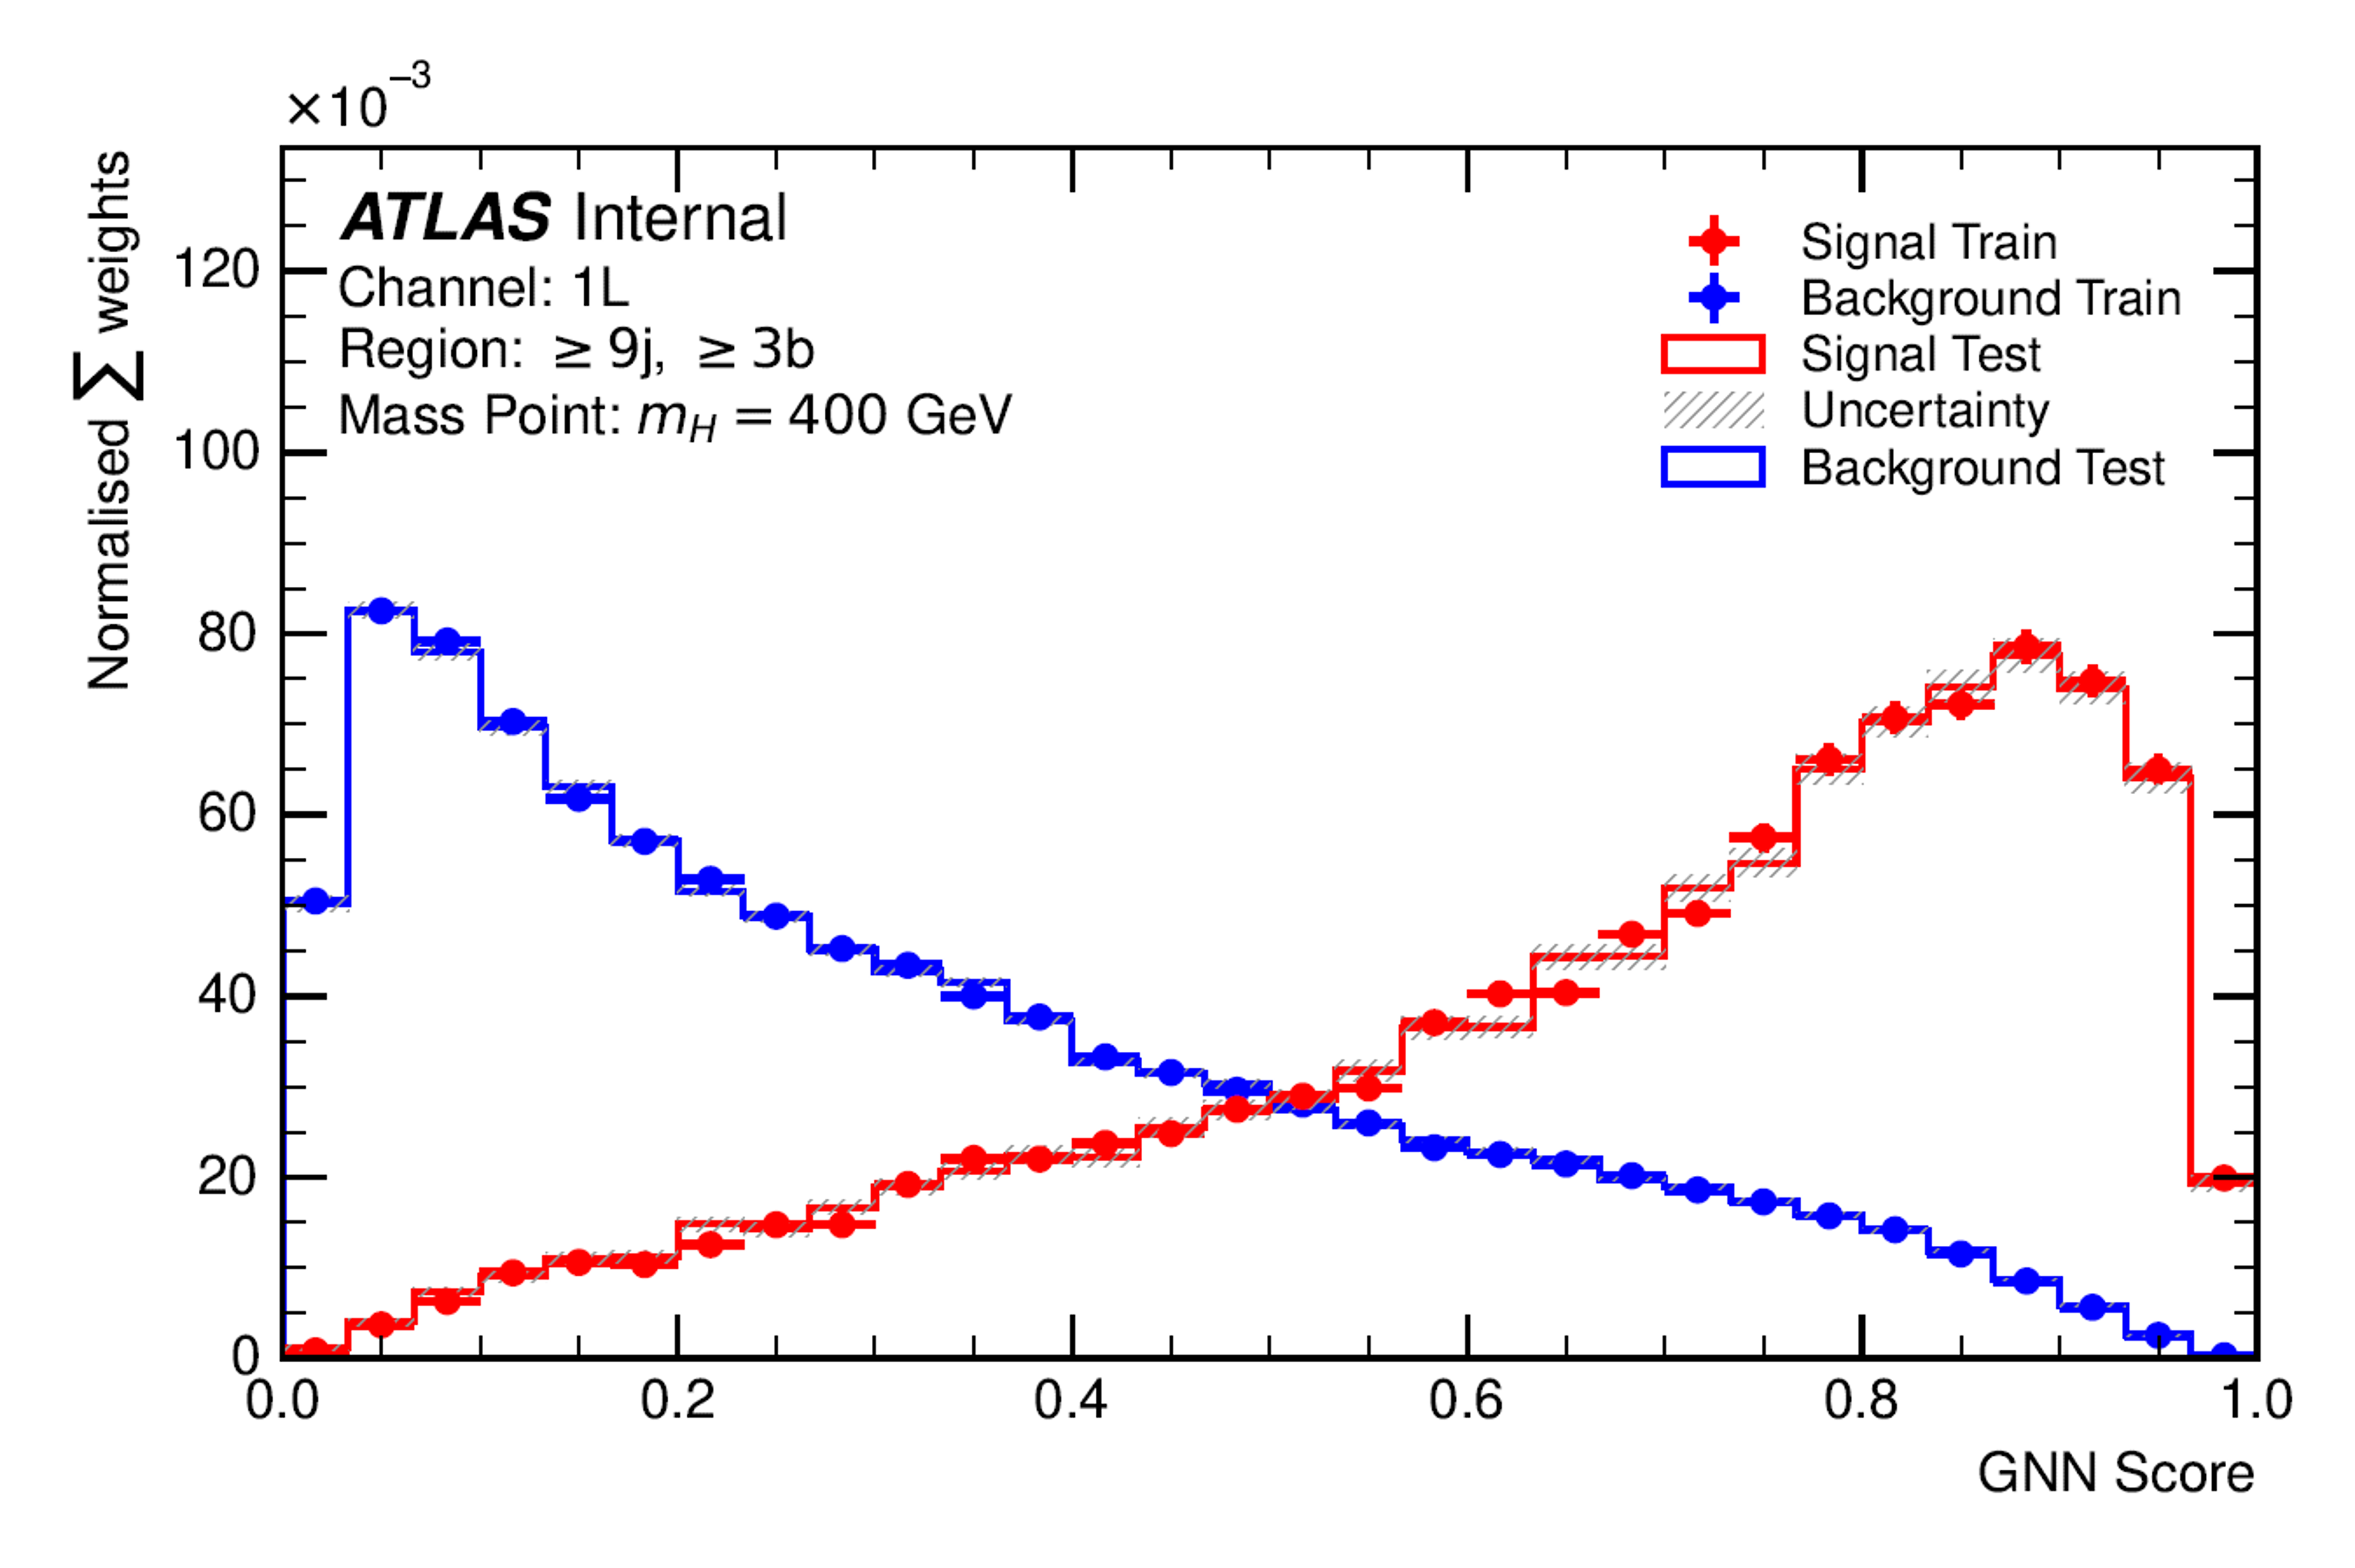
\includegraphics[width=0.48\textwidth]{figures/gnn/Plots_1L/400/GNN_Score_Plot_400GeV_Inclusive.png}
        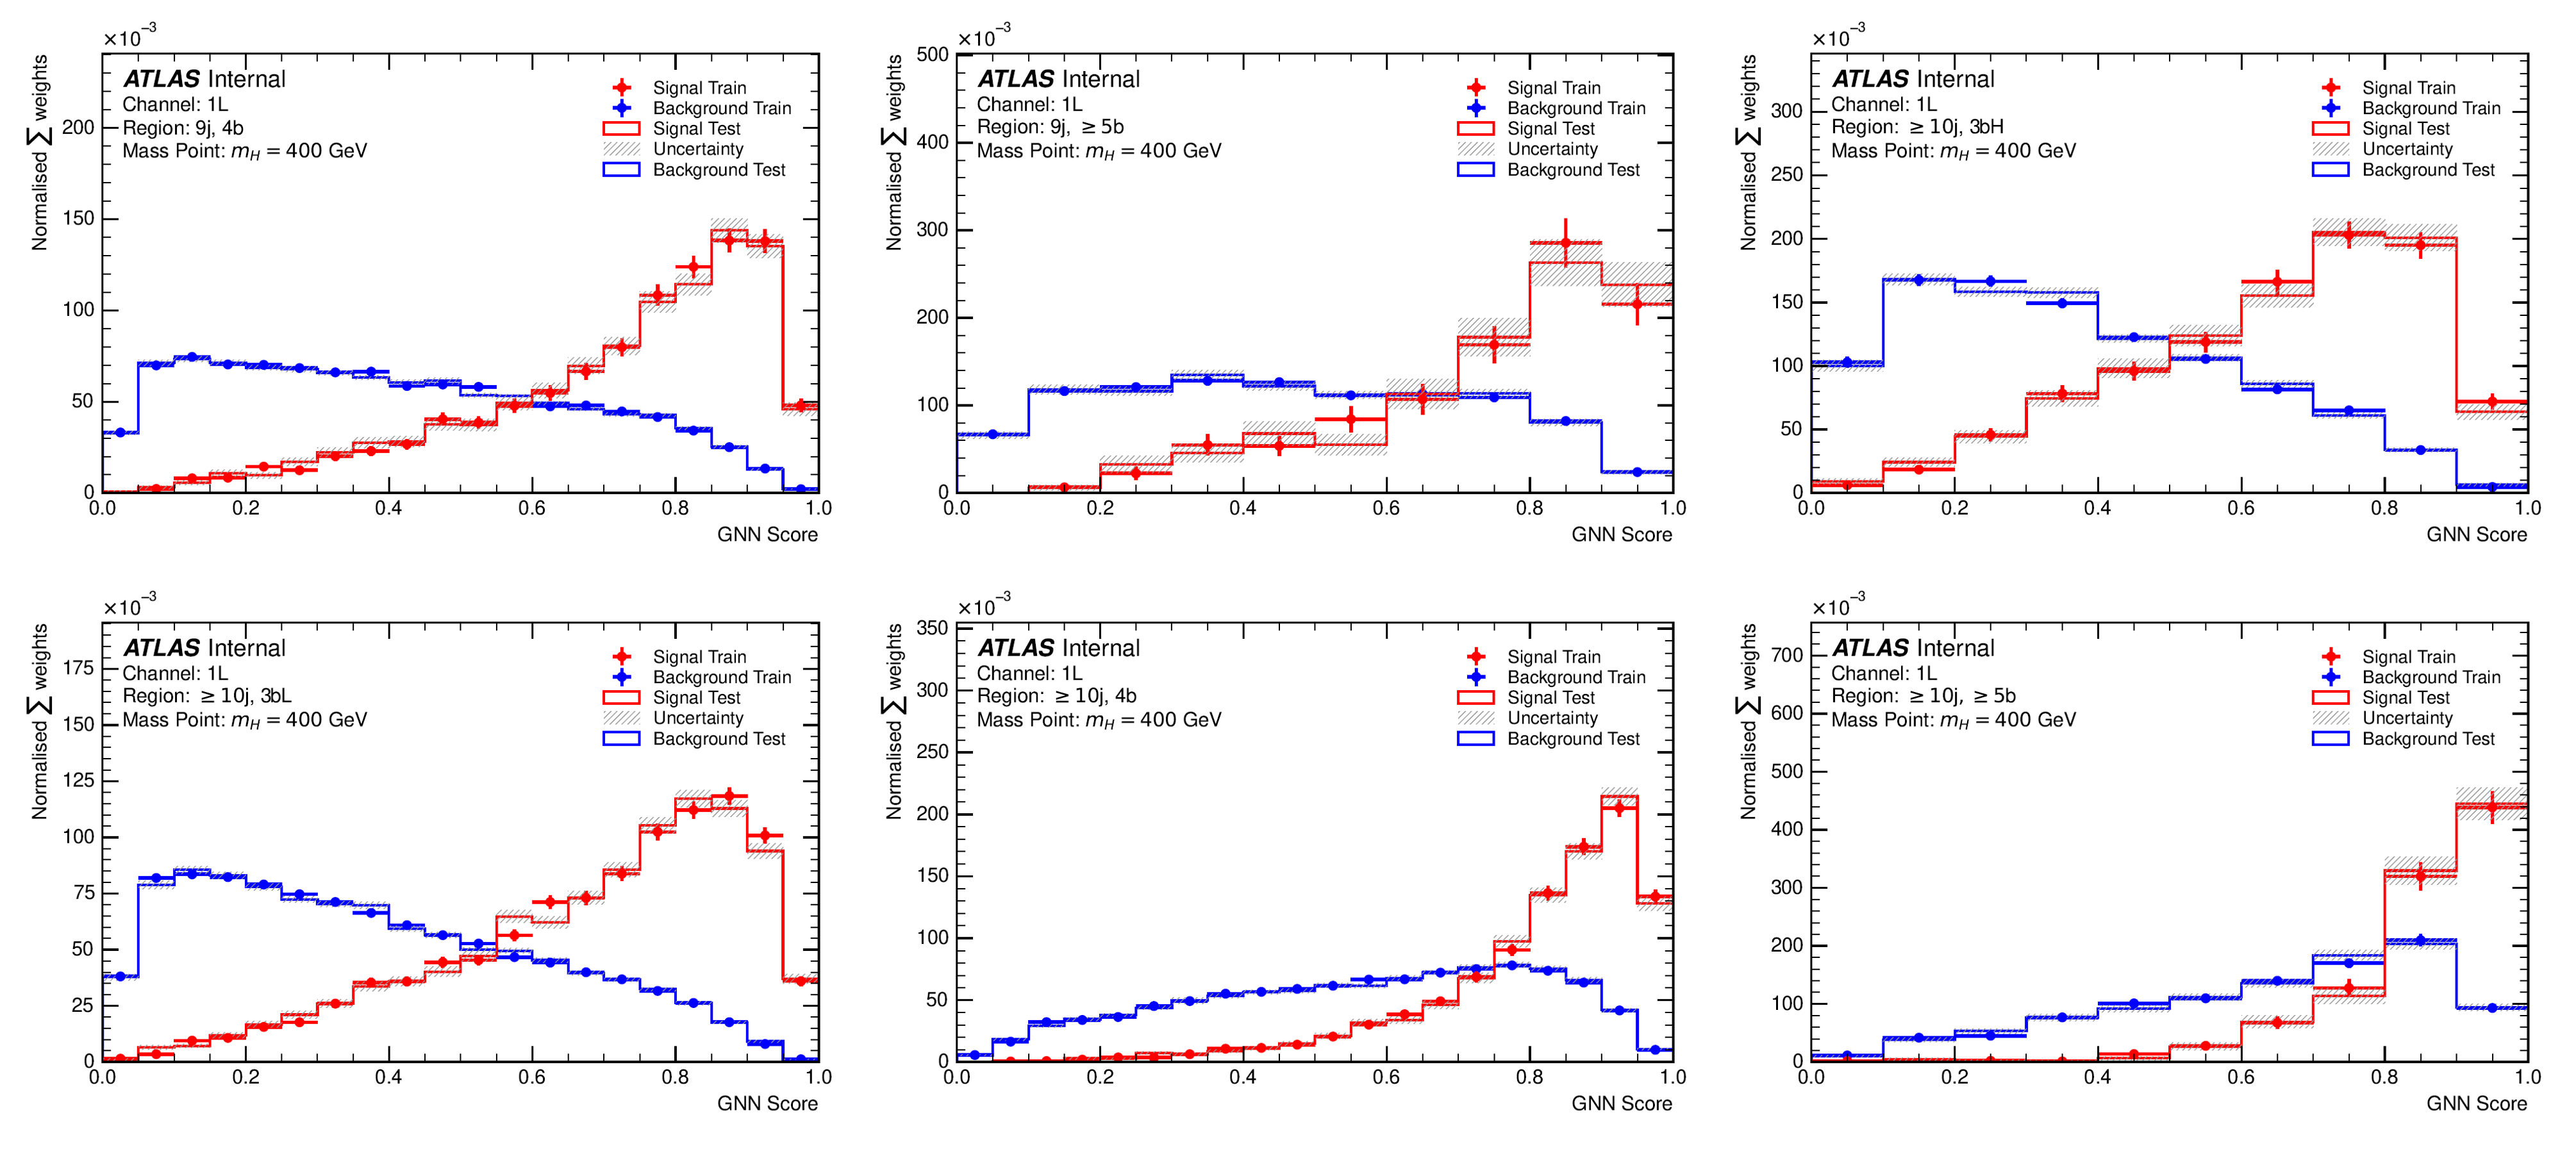
\includegraphics[width=0.48\textwidth]{figures/gnn/Plots_1L/400/GNN_Score_Plot_400GeV_Split.png}
        \caption{400 GeV mass point}
    \end{subfigure}
    \bigskip
    \centering
    \begin{subfigure}[t]{\textwidth}
        \centering
        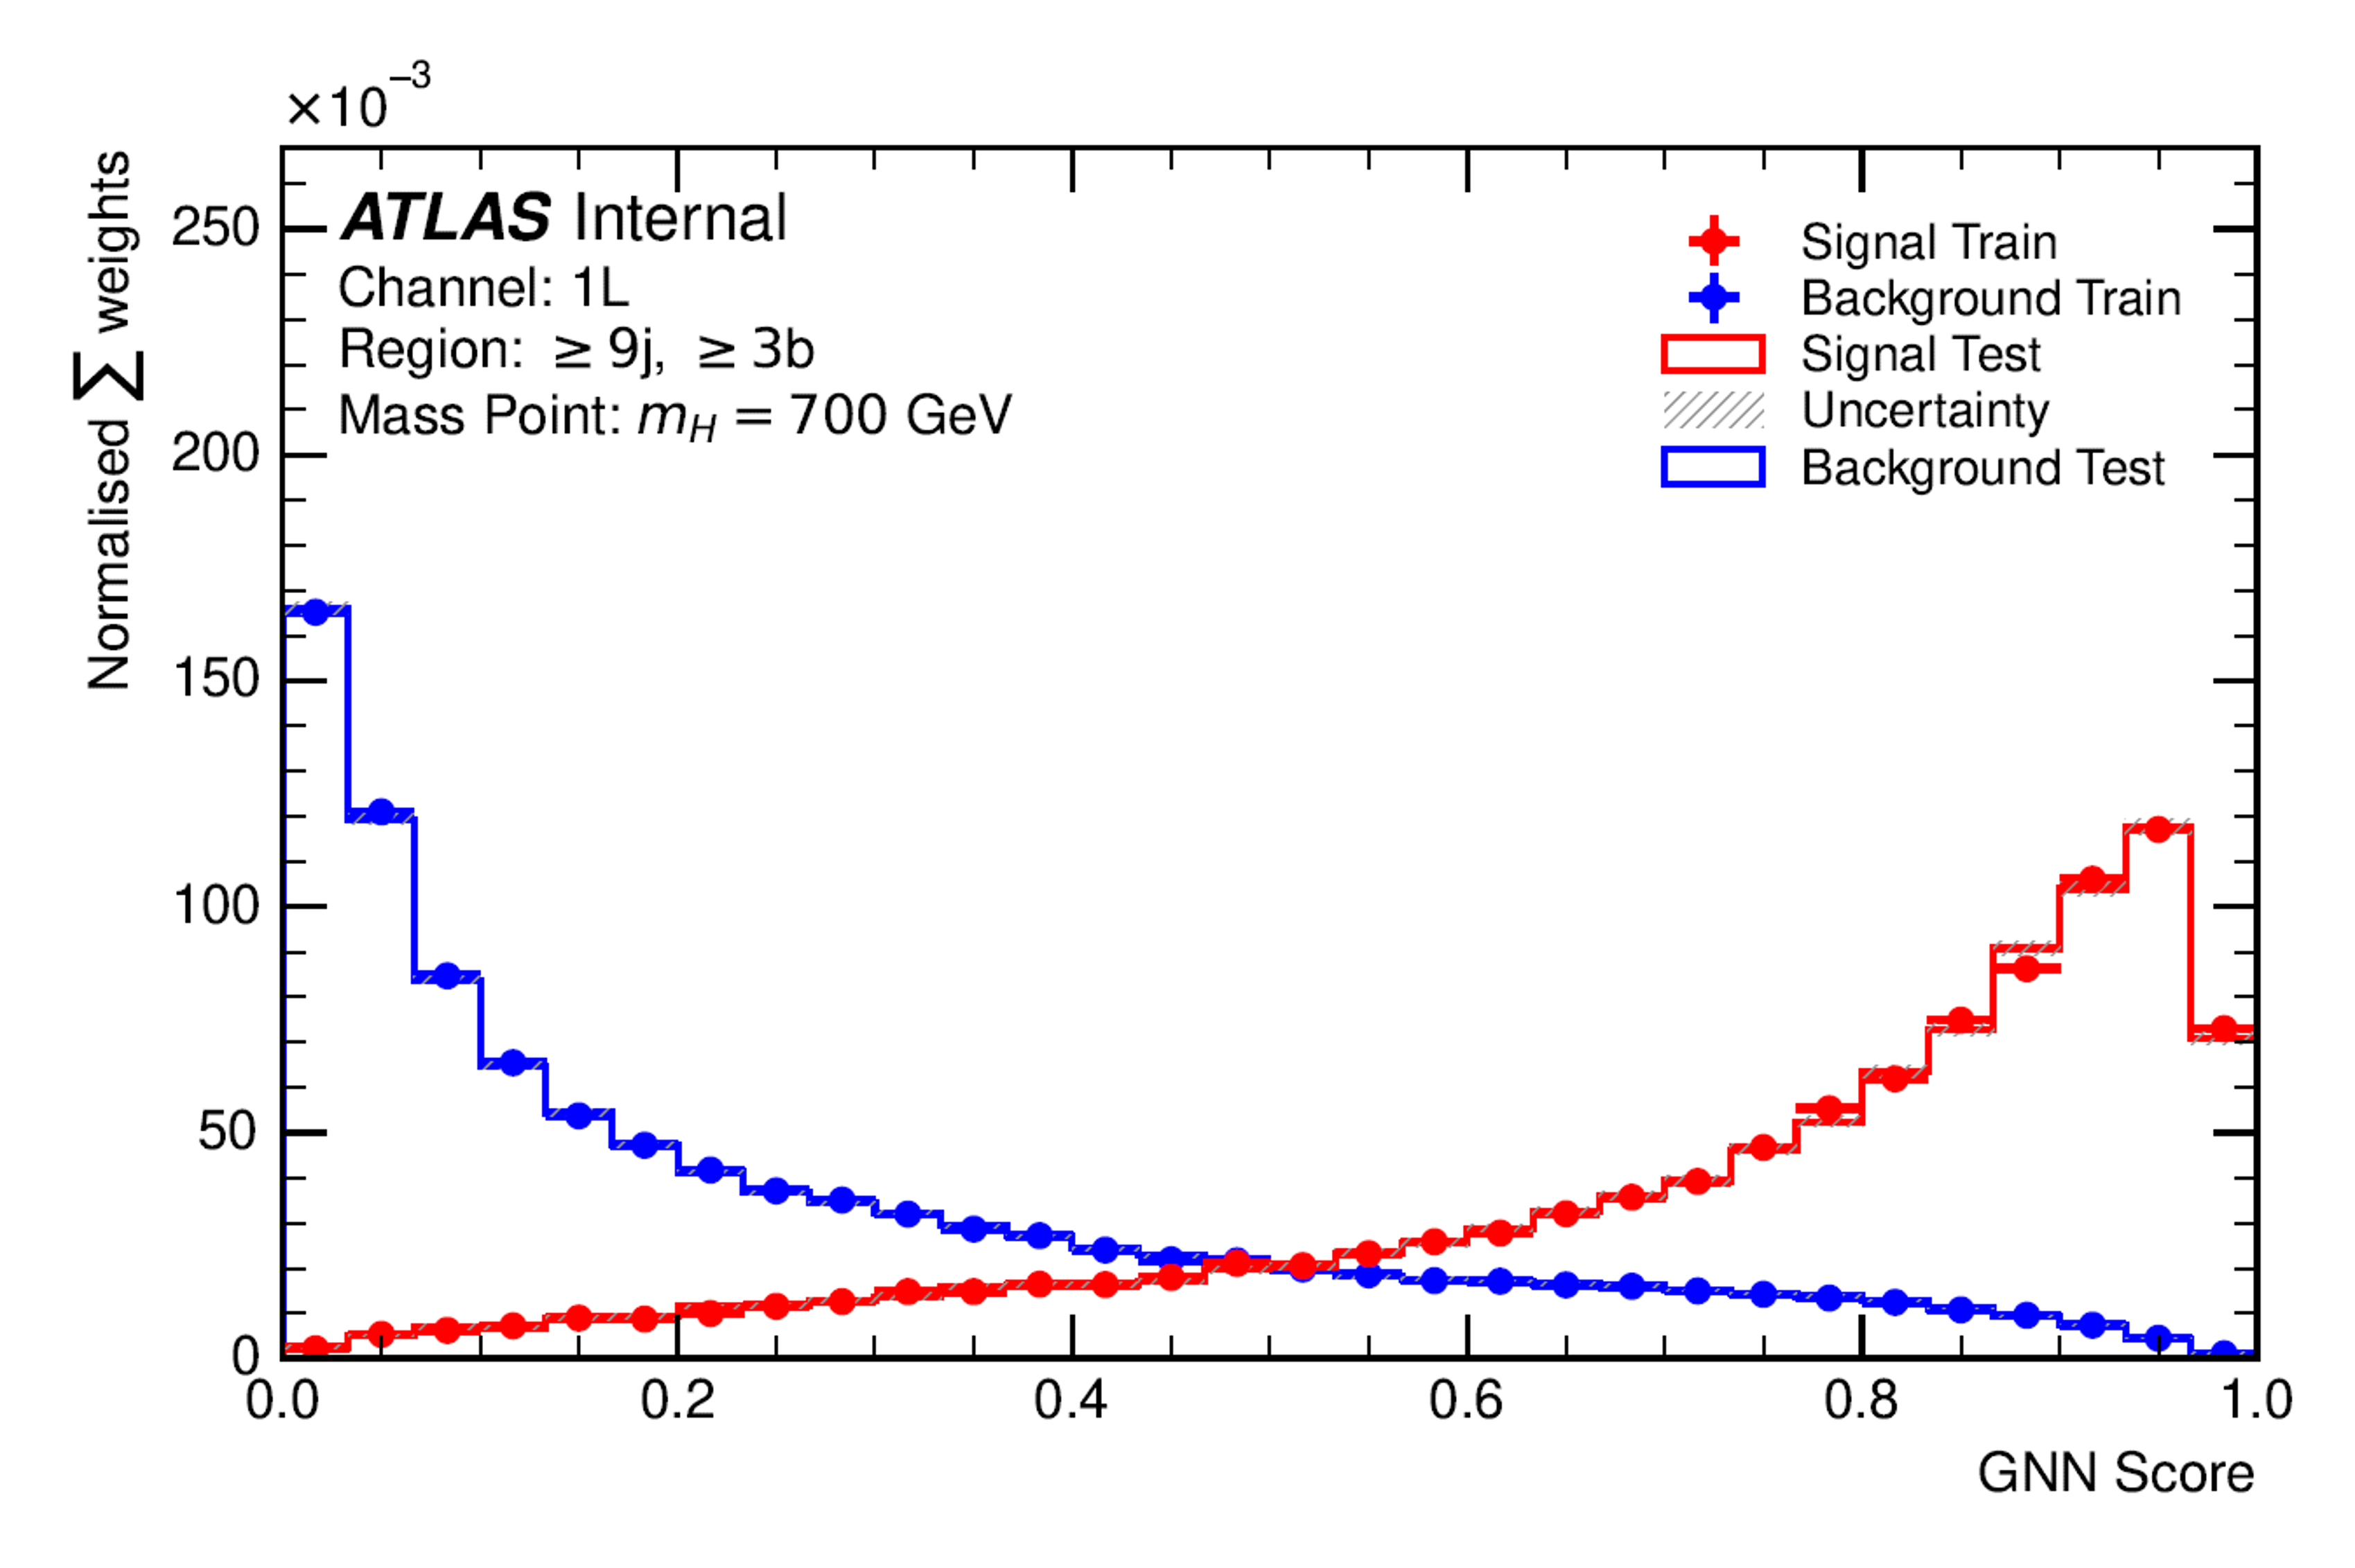
\includegraphics[width=0.48\textwidth]{figures/gnn/Plots_1L/700/GNN_Score_Plot_700GeV_Inclusive.png}
        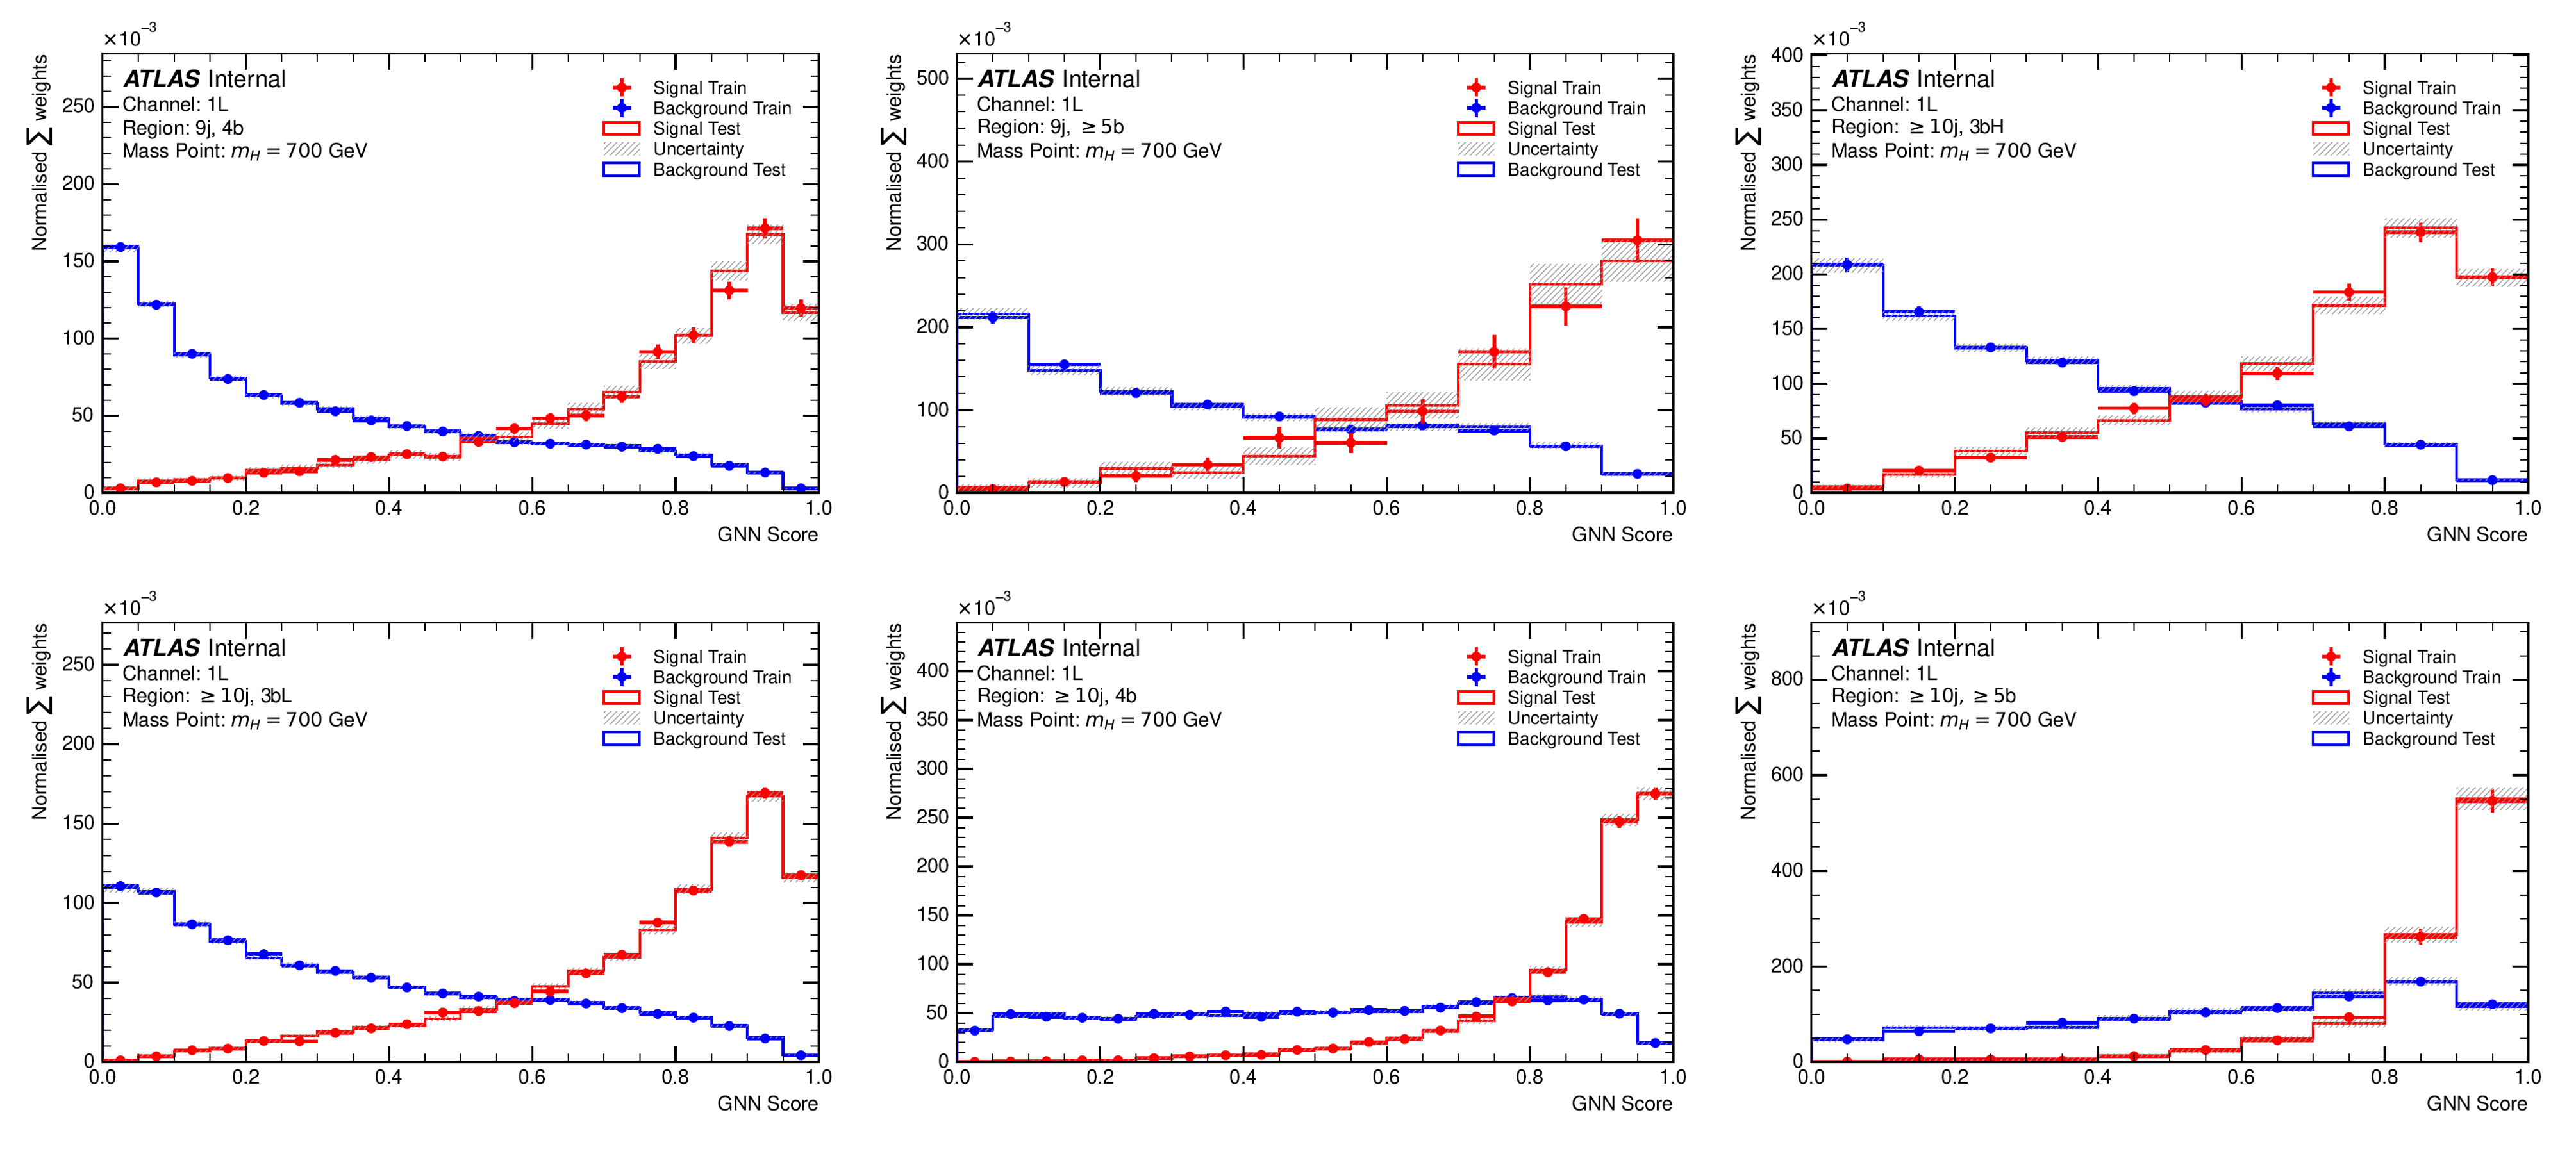
\includegraphics[width=0.48\textwidth]{figures/gnn/Plots_1L/700/GNN_Score_Plot_700GeV_Split.png}
        \caption{700 GeV mass point}
    \end{subfigure}
    \bigskip
    \centering
    \begin{subfigure}[t]{\textwidth}
        \centering
        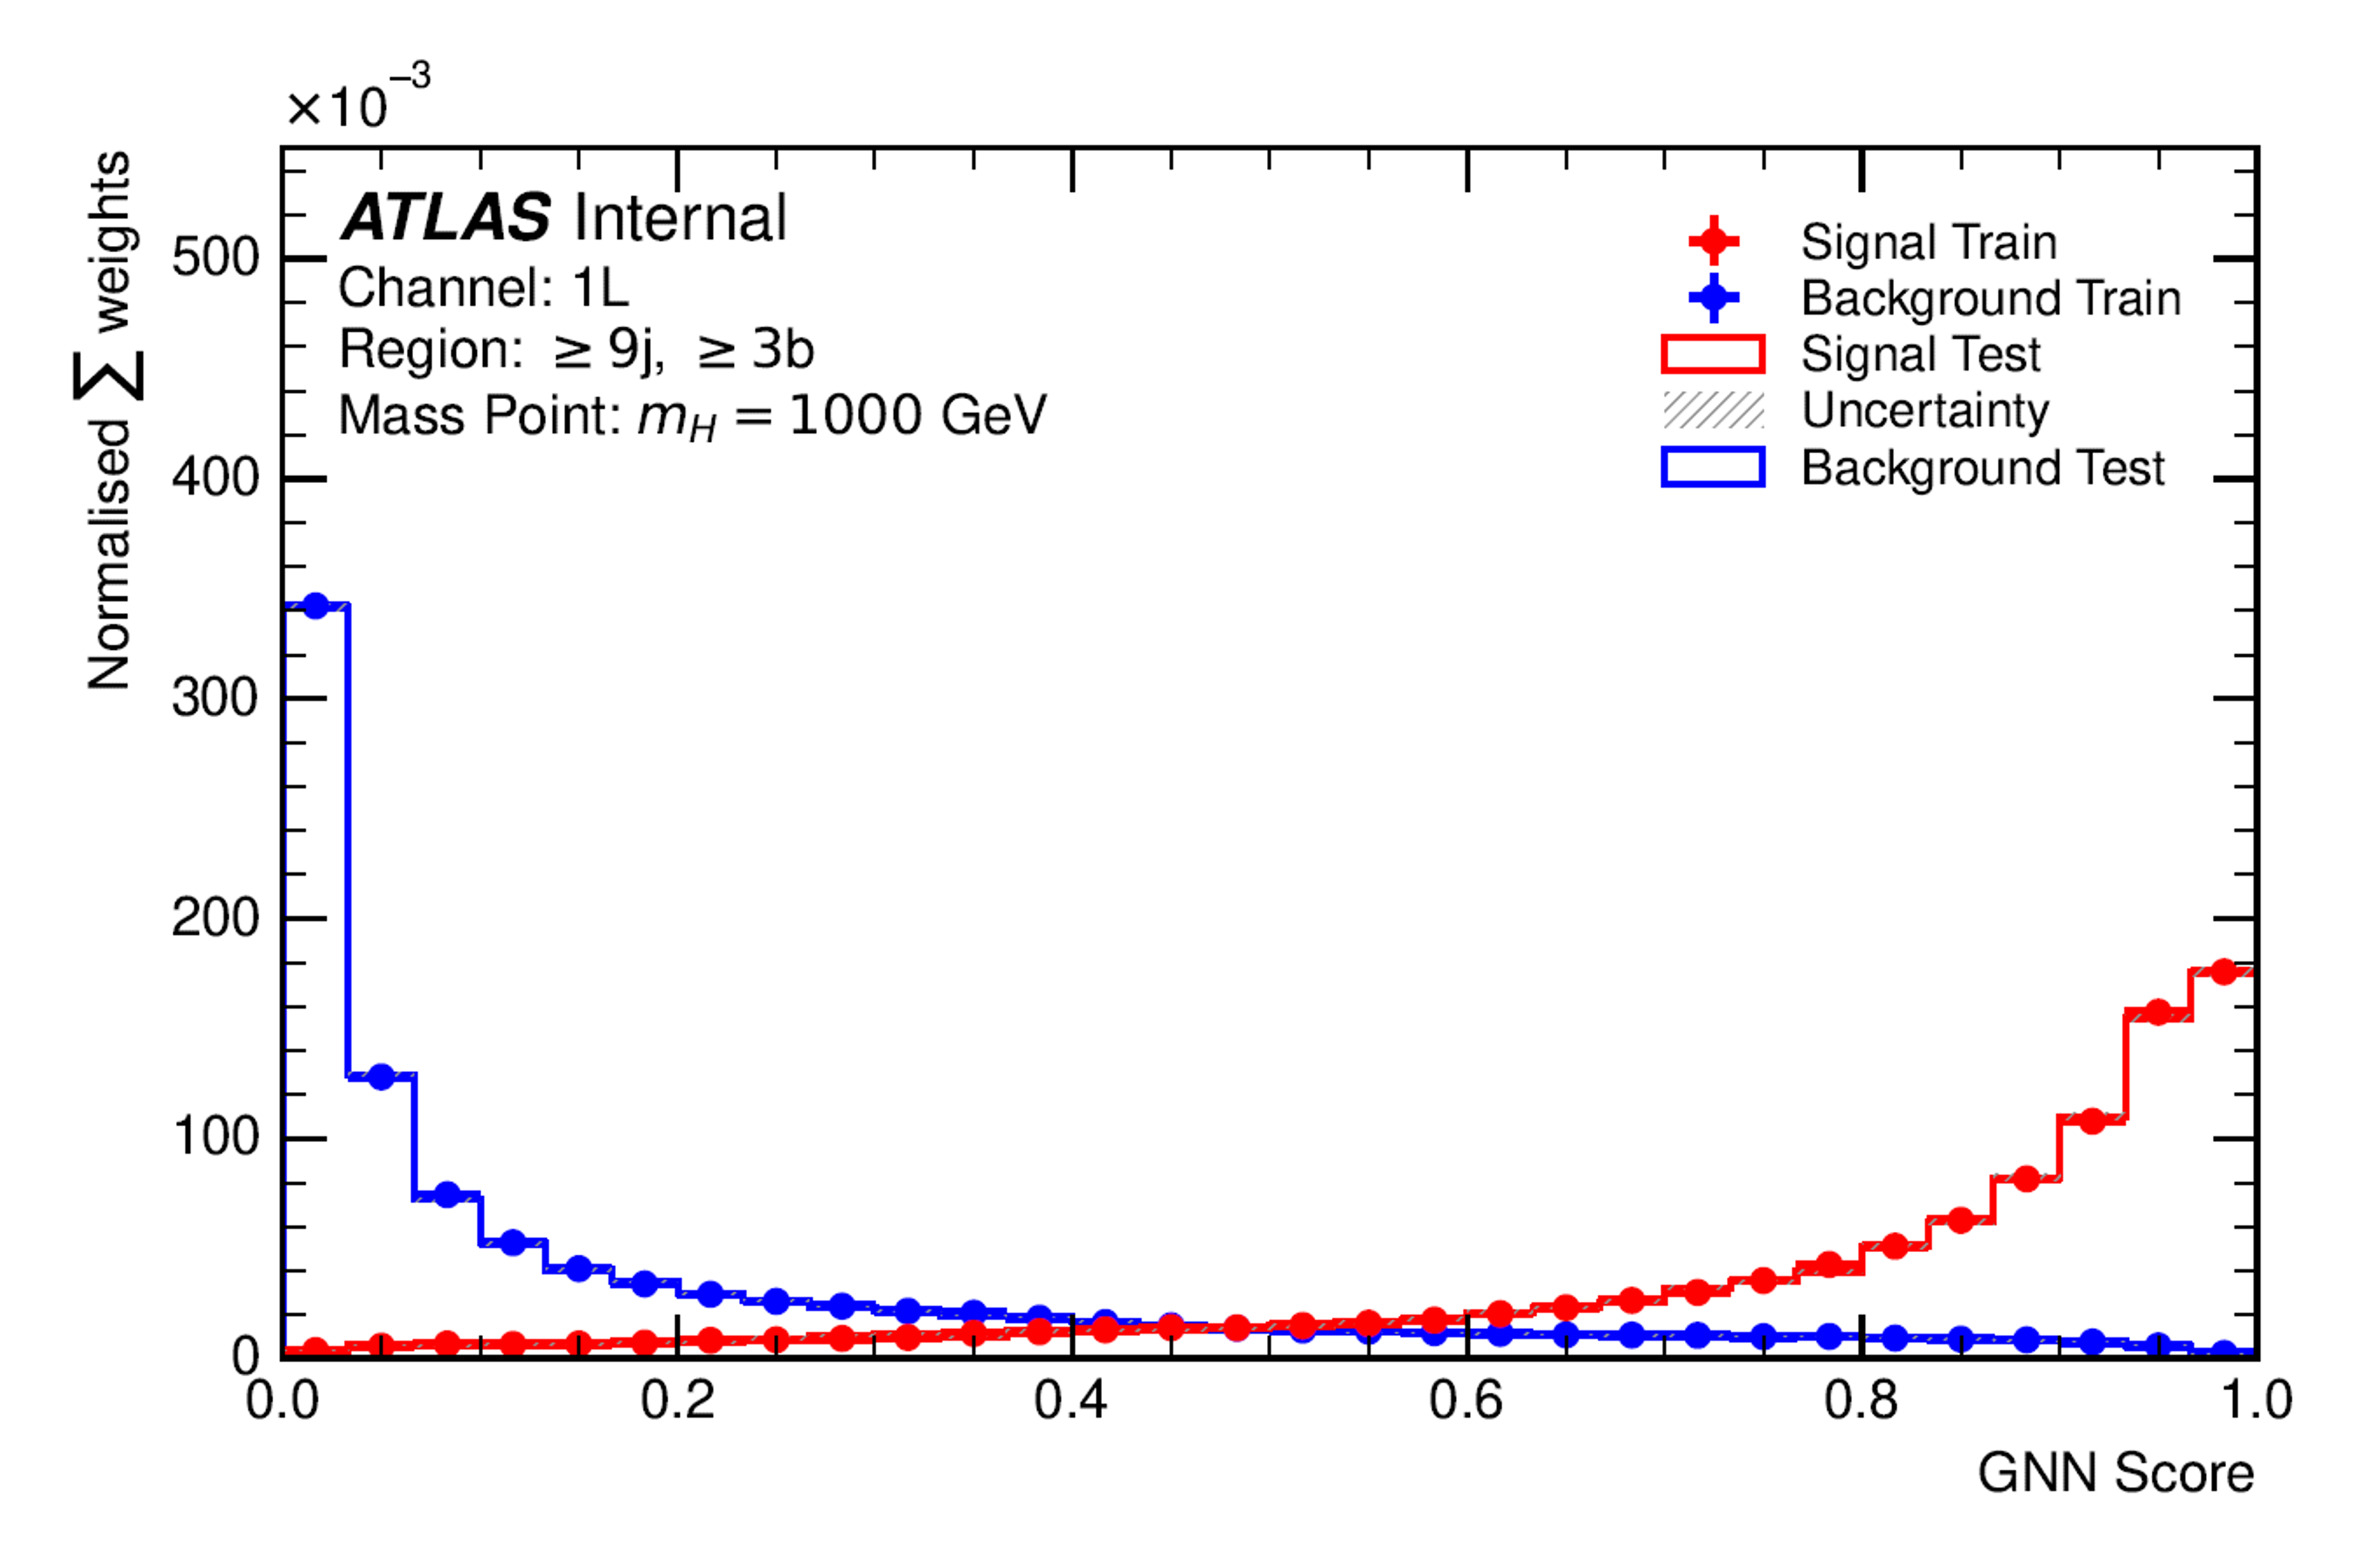
\includegraphics[width=0.48\textwidth]{figures/gnn/Plots_1L/1000/GNN_Score_Plot_1000GeV_Inclusive.png}
        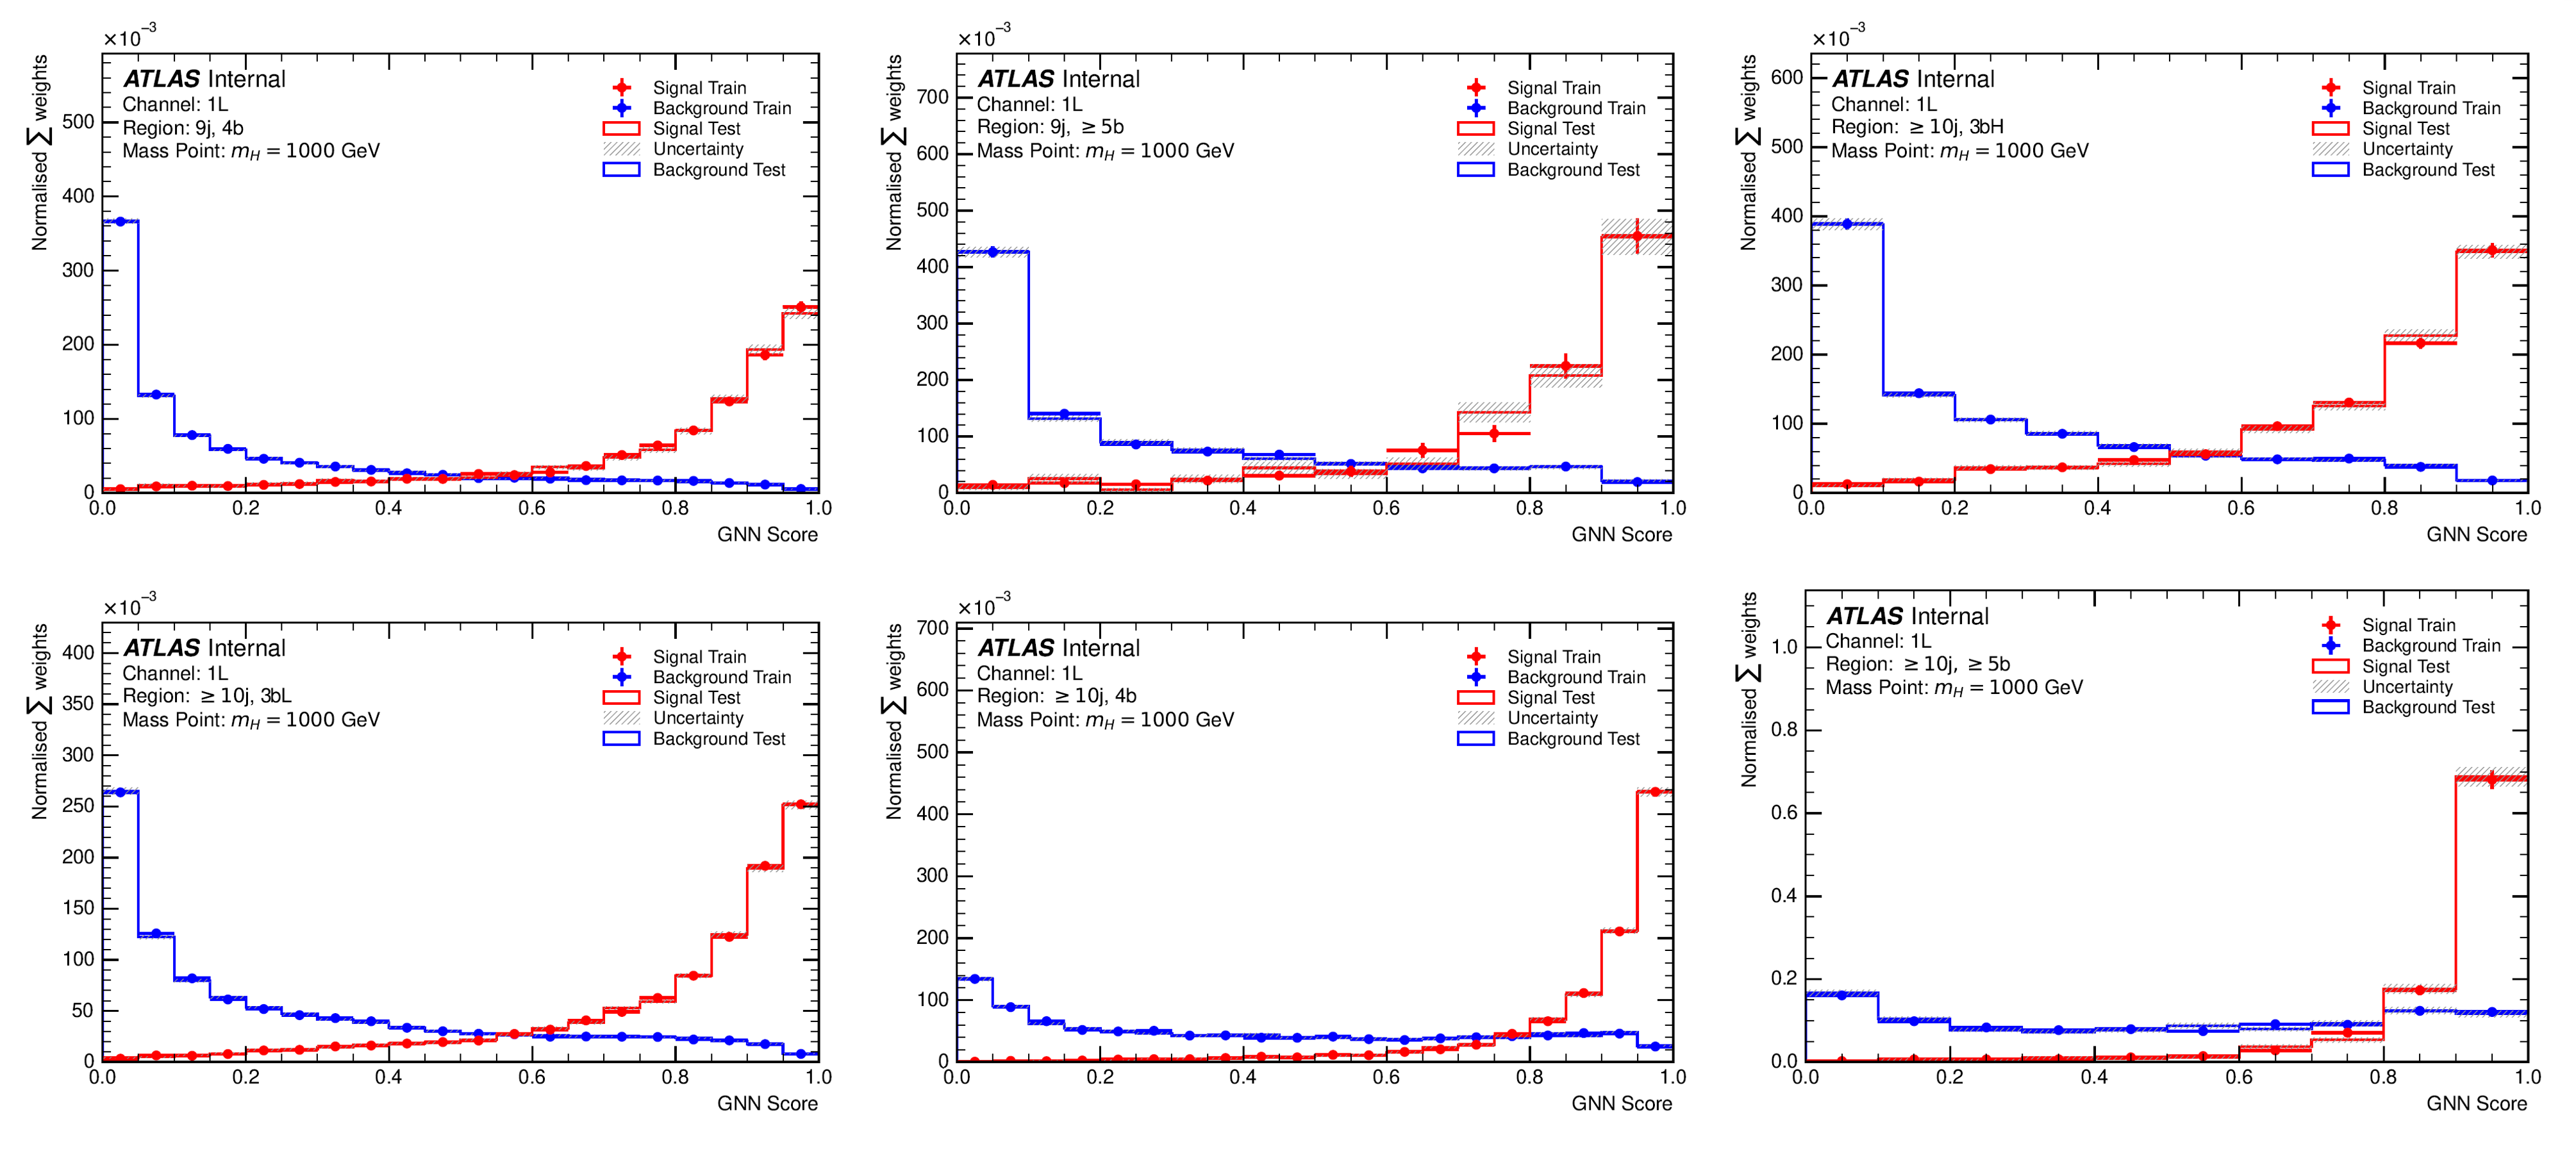
\includegraphics[width=0.48\textwidth]{figures/gnn/Plots_1L/1000/GNN_Score_Plot_1000GeV_Split.png}
        \caption{1000 GeV mass point}
    \end{subfigure}
    \caption{Score distributions for the 1L GNN for several mass points. Shown in the inclusive training region (left) and four subdivided regions (right). Distributions are shown separately for models trained on even/odd event numbers and are split into training and testing results. The combined result of the cross trained model is shown in blue (signal) and red (background).}
    \label{fig:1l-gnn-scores}
\end{figure} 


\begin{figure}[h!]
    \centering
    \begin{subfigure}[t]{\textwidth}
        \centering
        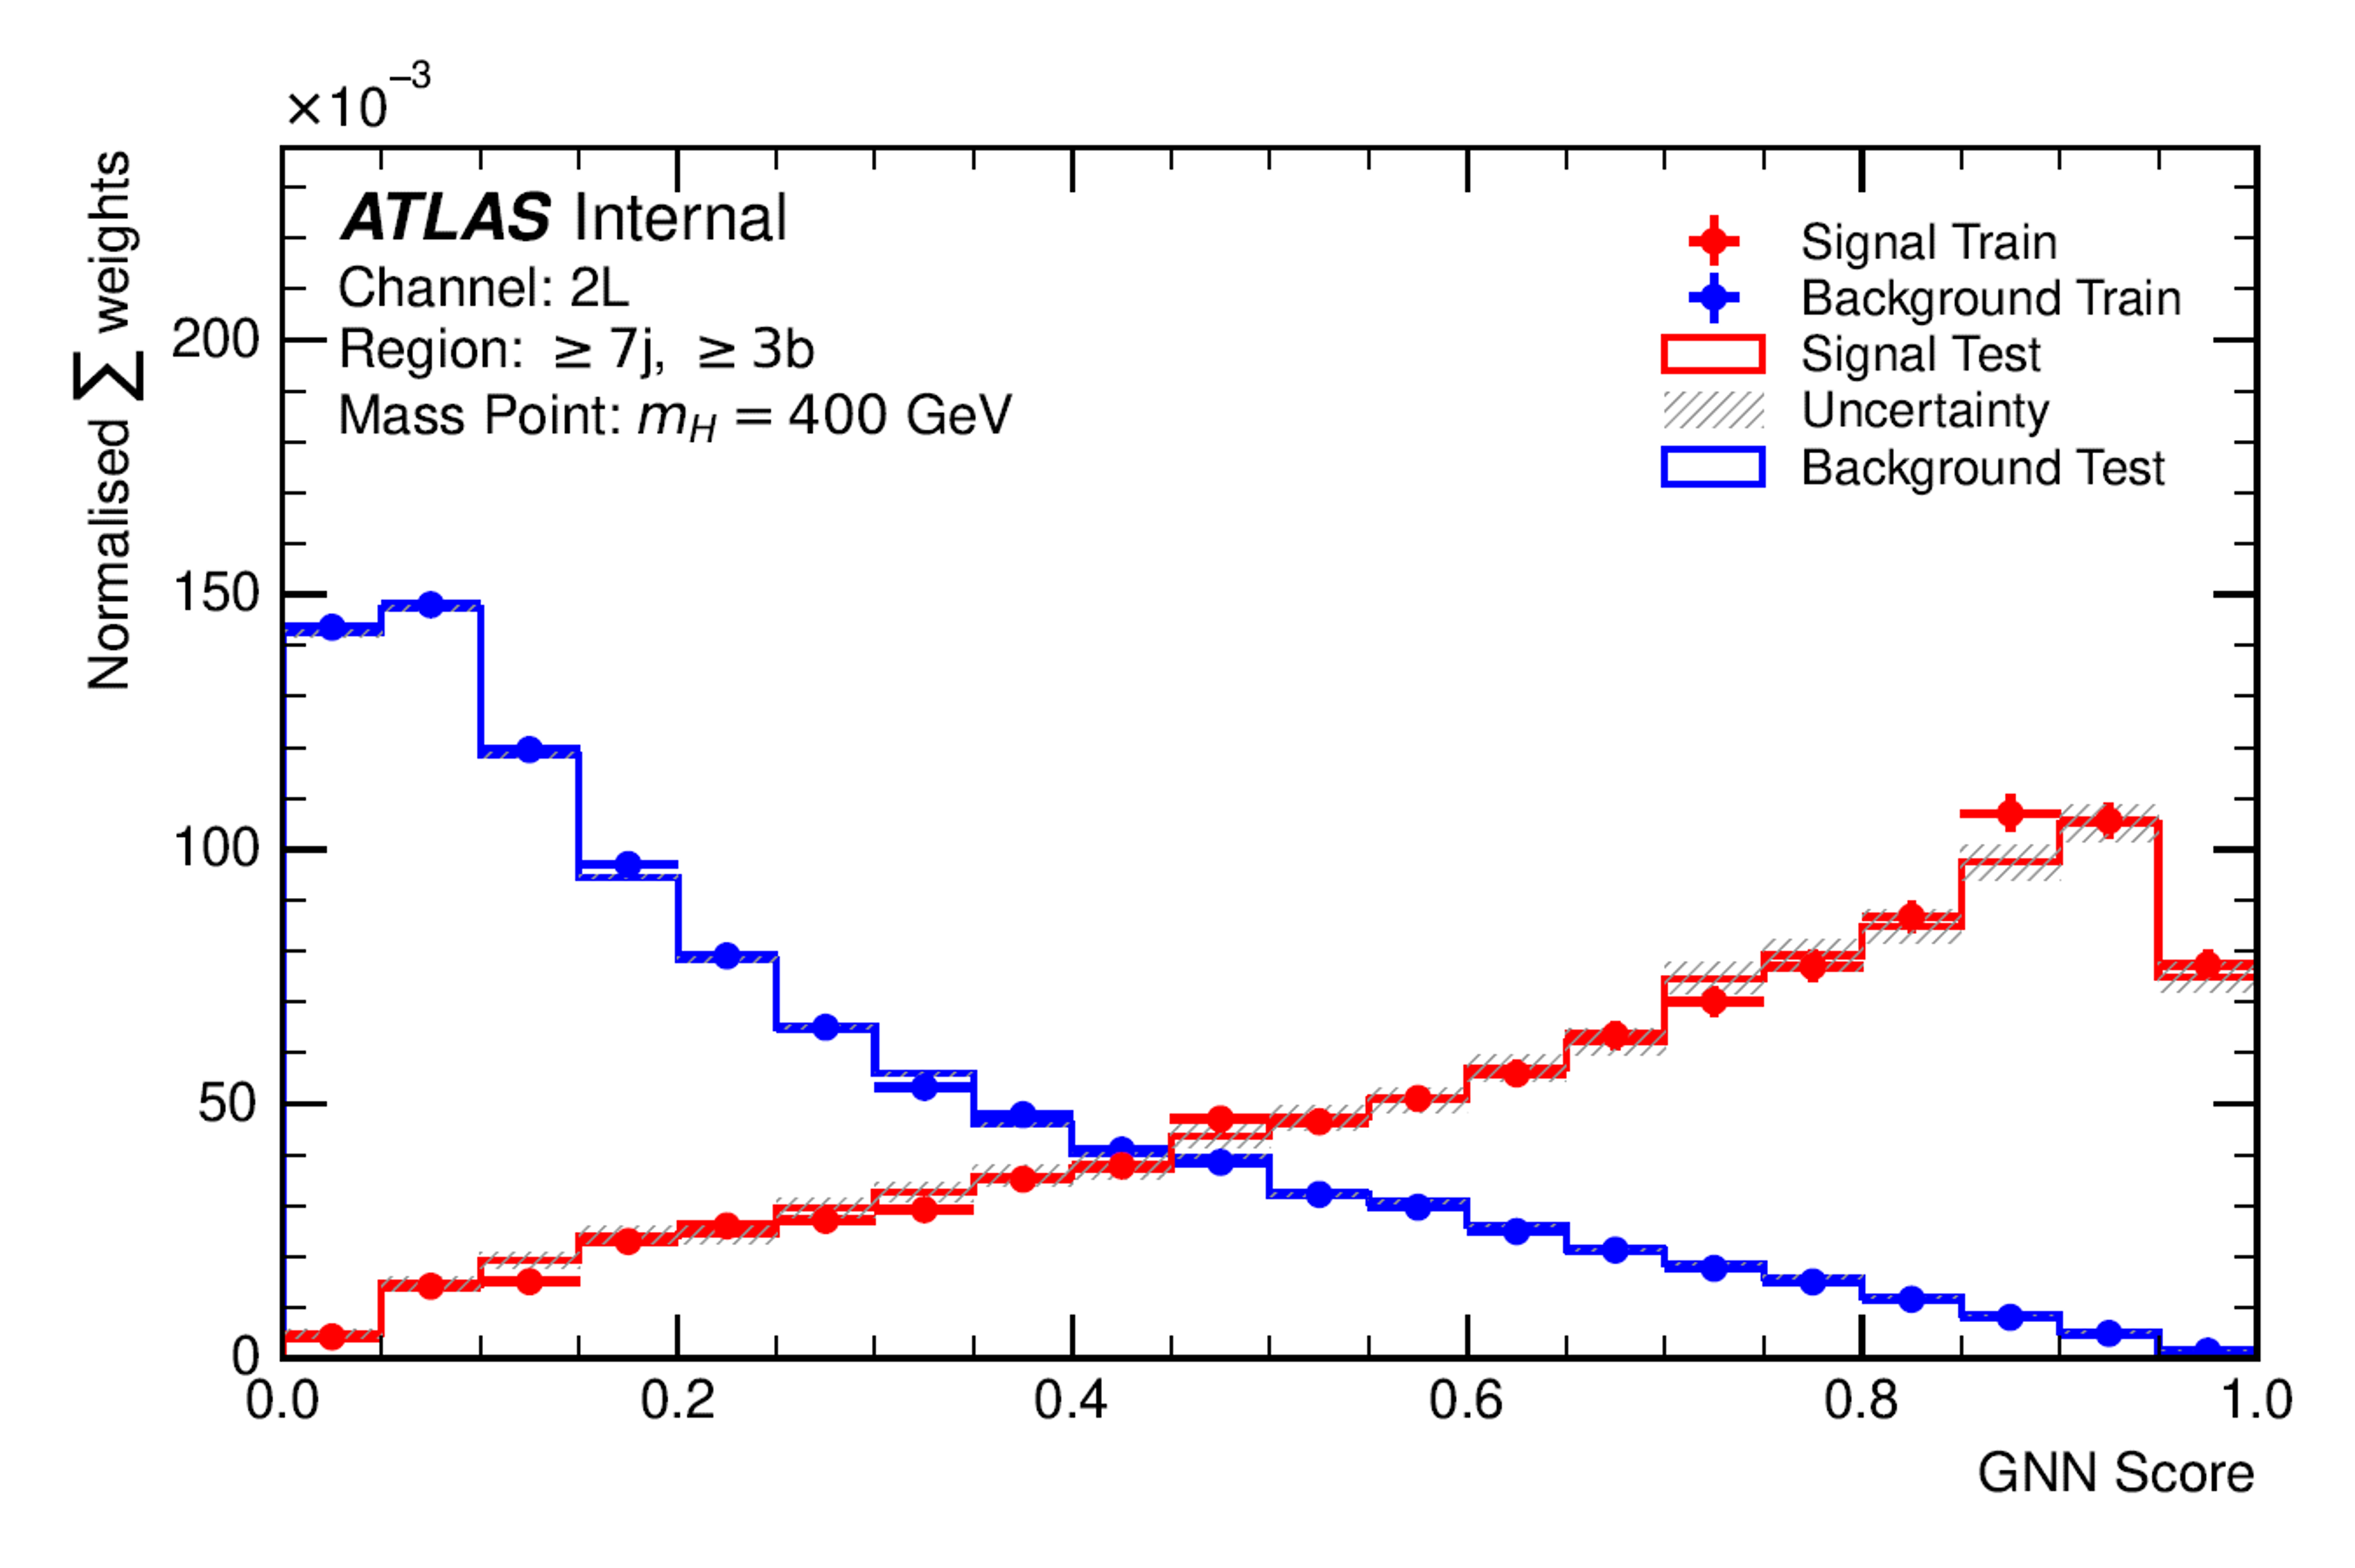
\includegraphics[width=0.48\textwidth]{figures/gnn/Plots_2LOS/400/GNN_Score_Plot_400GeV_Inclusive.png}
        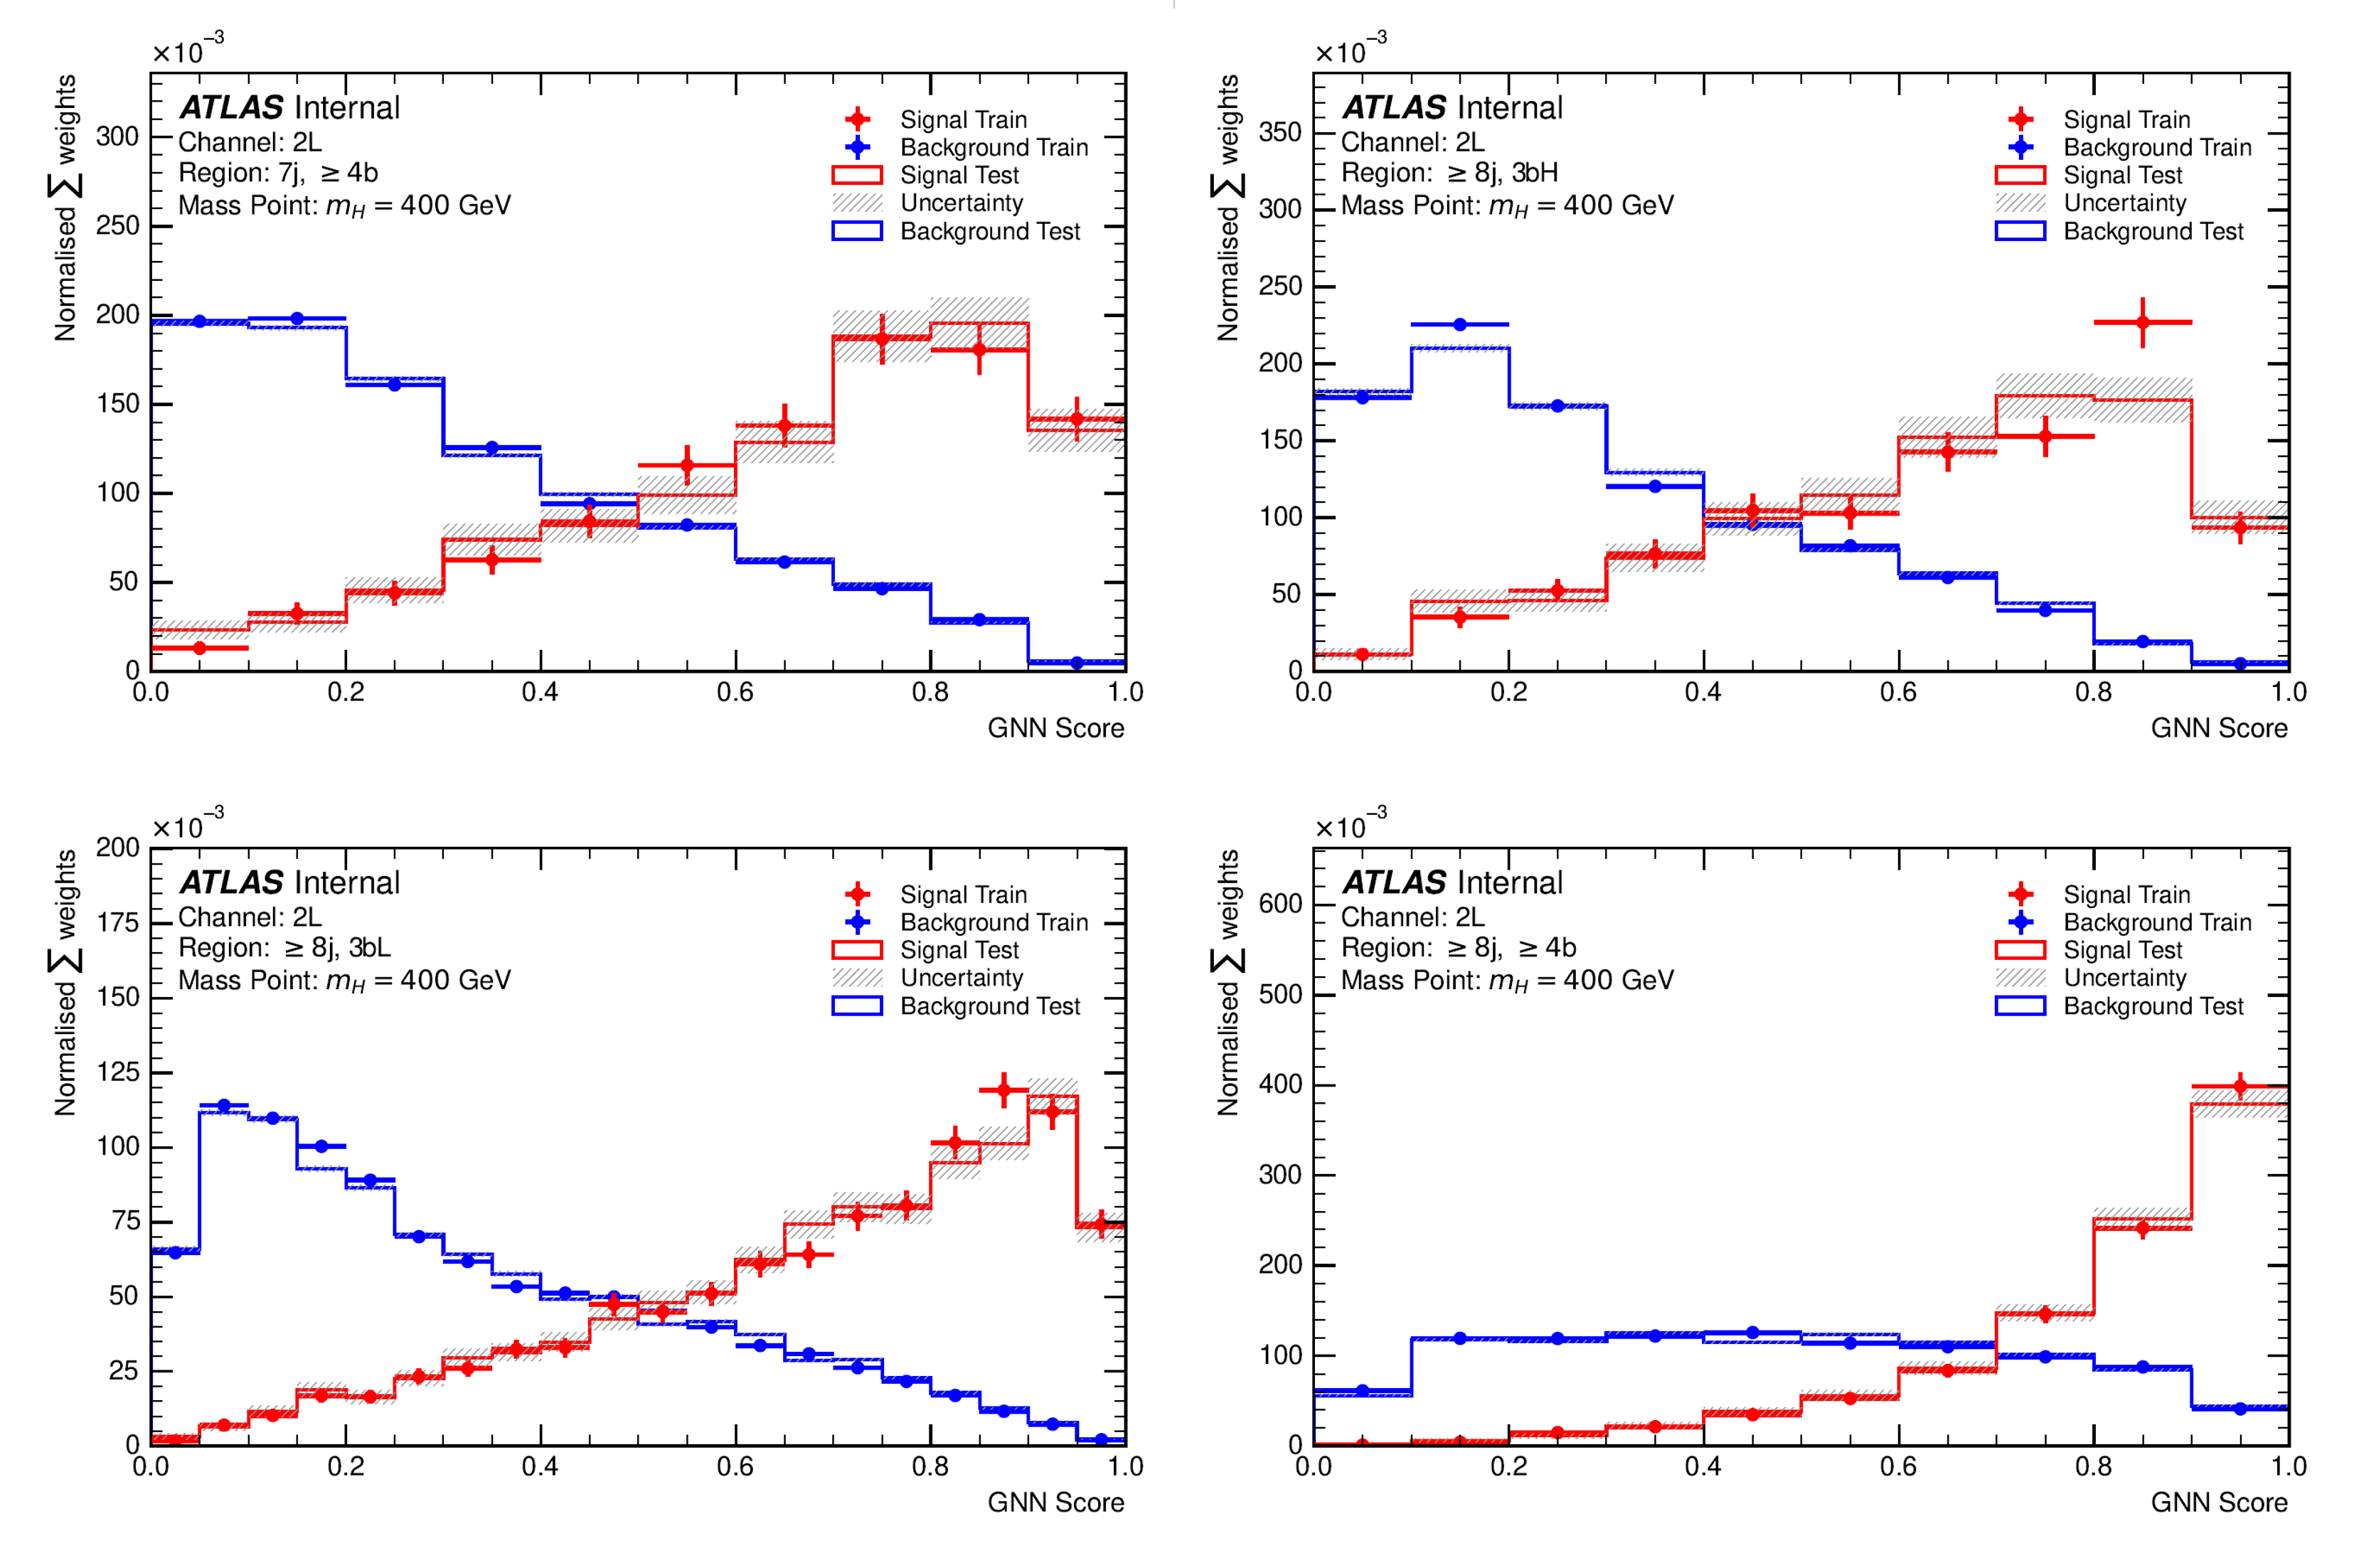
\includegraphics[width=0.48\textwidth]{figures/gnn/Plots_2LOS/400/GNN_Score_Plot_400GeV_Split.png}
        \caption{400 GeV mass point}
    \end{subfigure}
    \bigskip
    \centering
    \begin{subfigure}[t]{\textwidth}
        \centering
        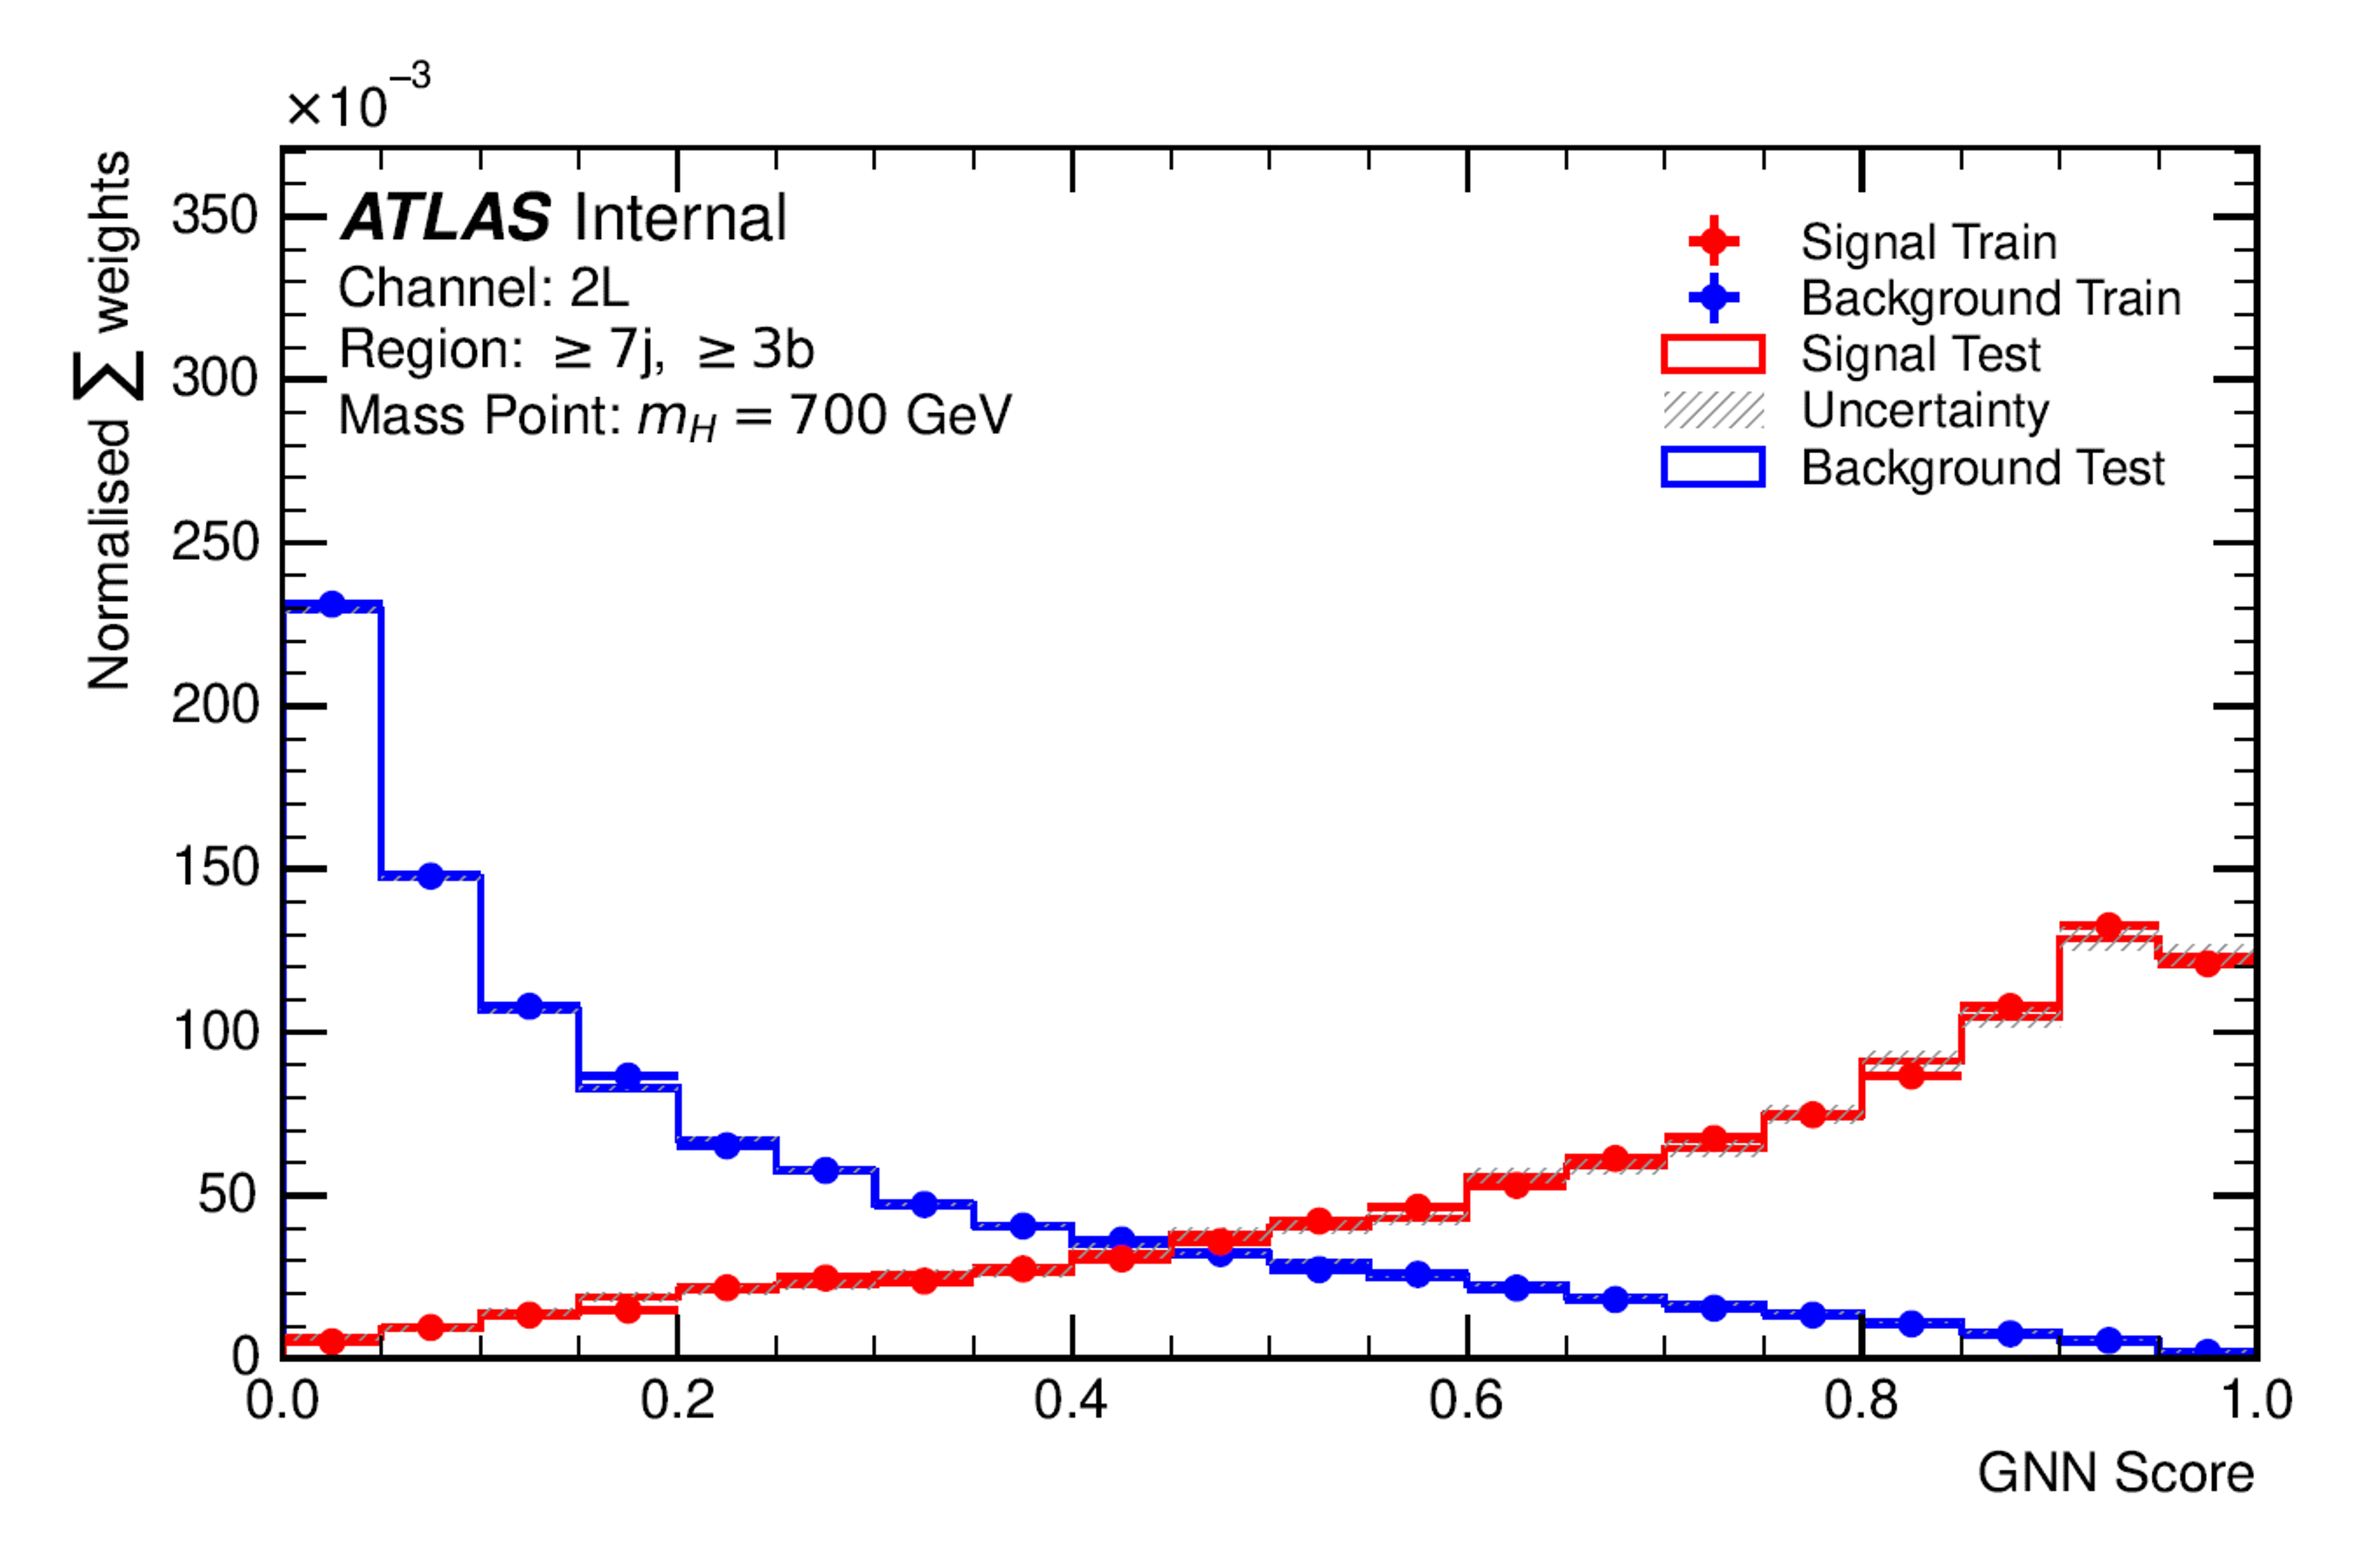
\includegraphics[width=.48\textwidth]{figures/gnn/Plots_2LOS/700/GNN_Score_Plot_700GeV_Inclusive.png}
        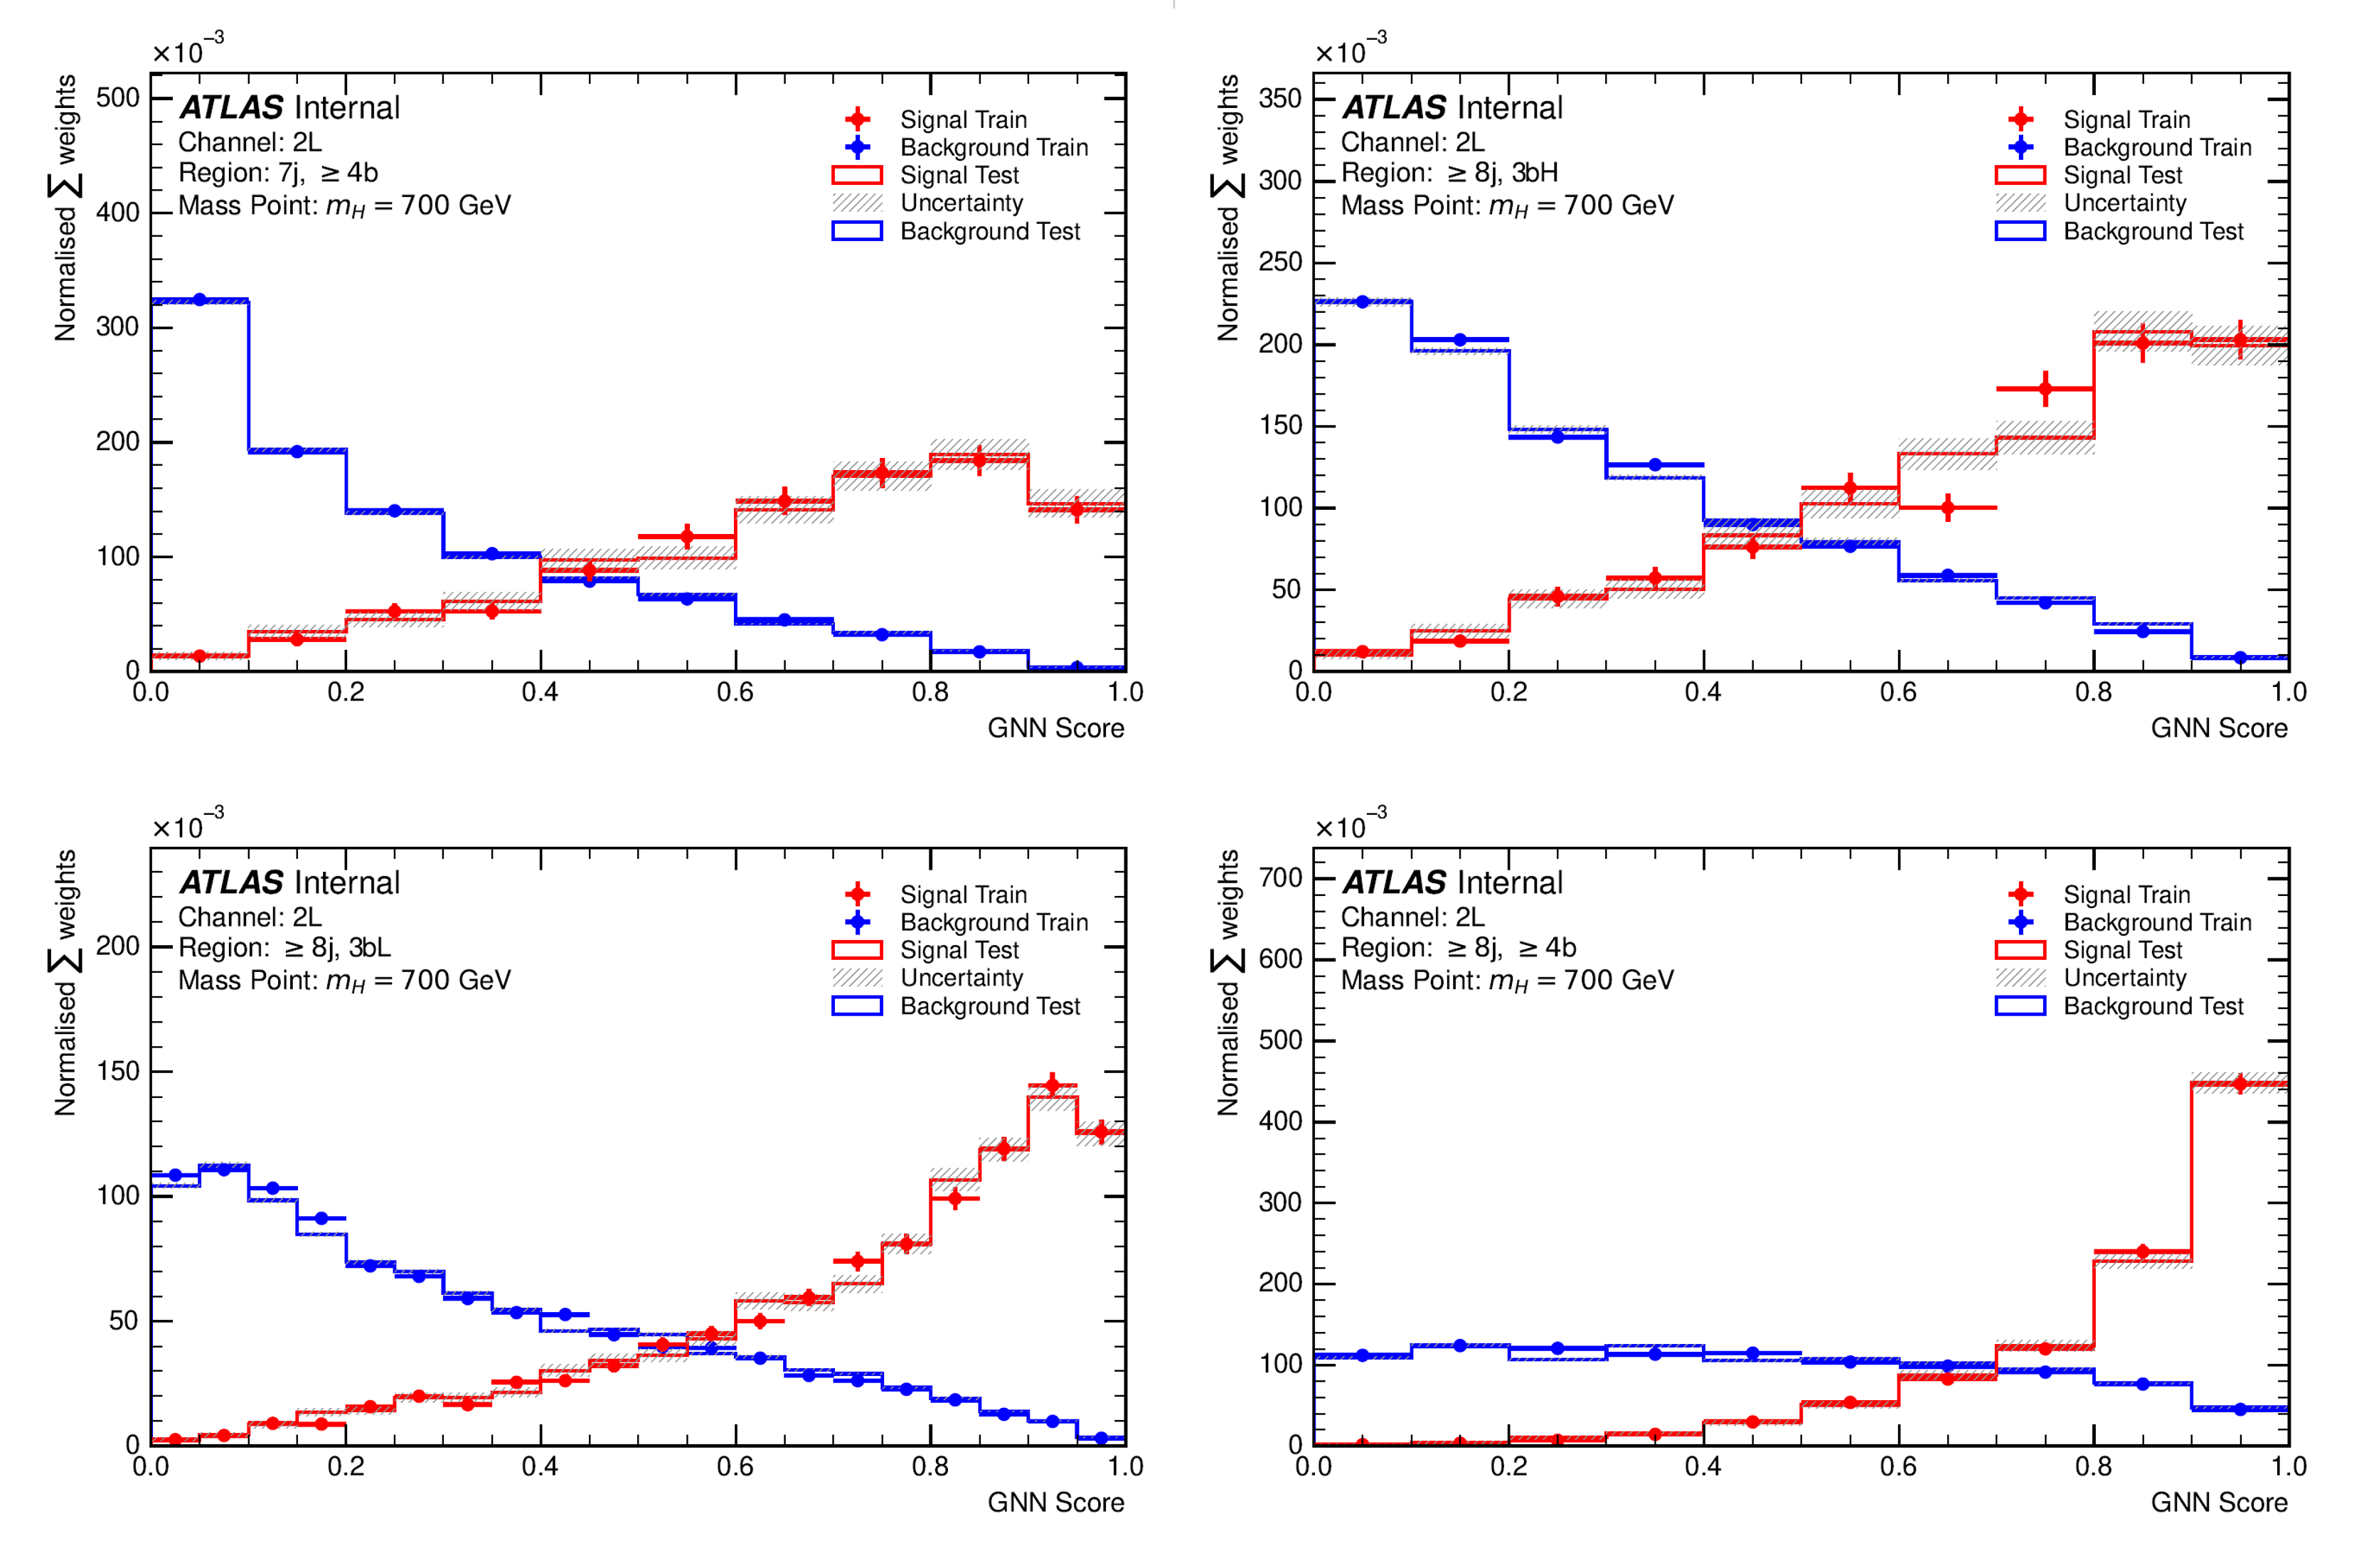
\includegraphics[width=.48\textwidth]{figures/gnn/Plots_2LOS/700/GNN_Score_Plot_700GeV_Split.png}
        \caption{700 GeV mass point}
    \end{subfigure}
    \bigskip
    \centering
    \begin{subfigure}[t]{\textwidth}
        \centering
        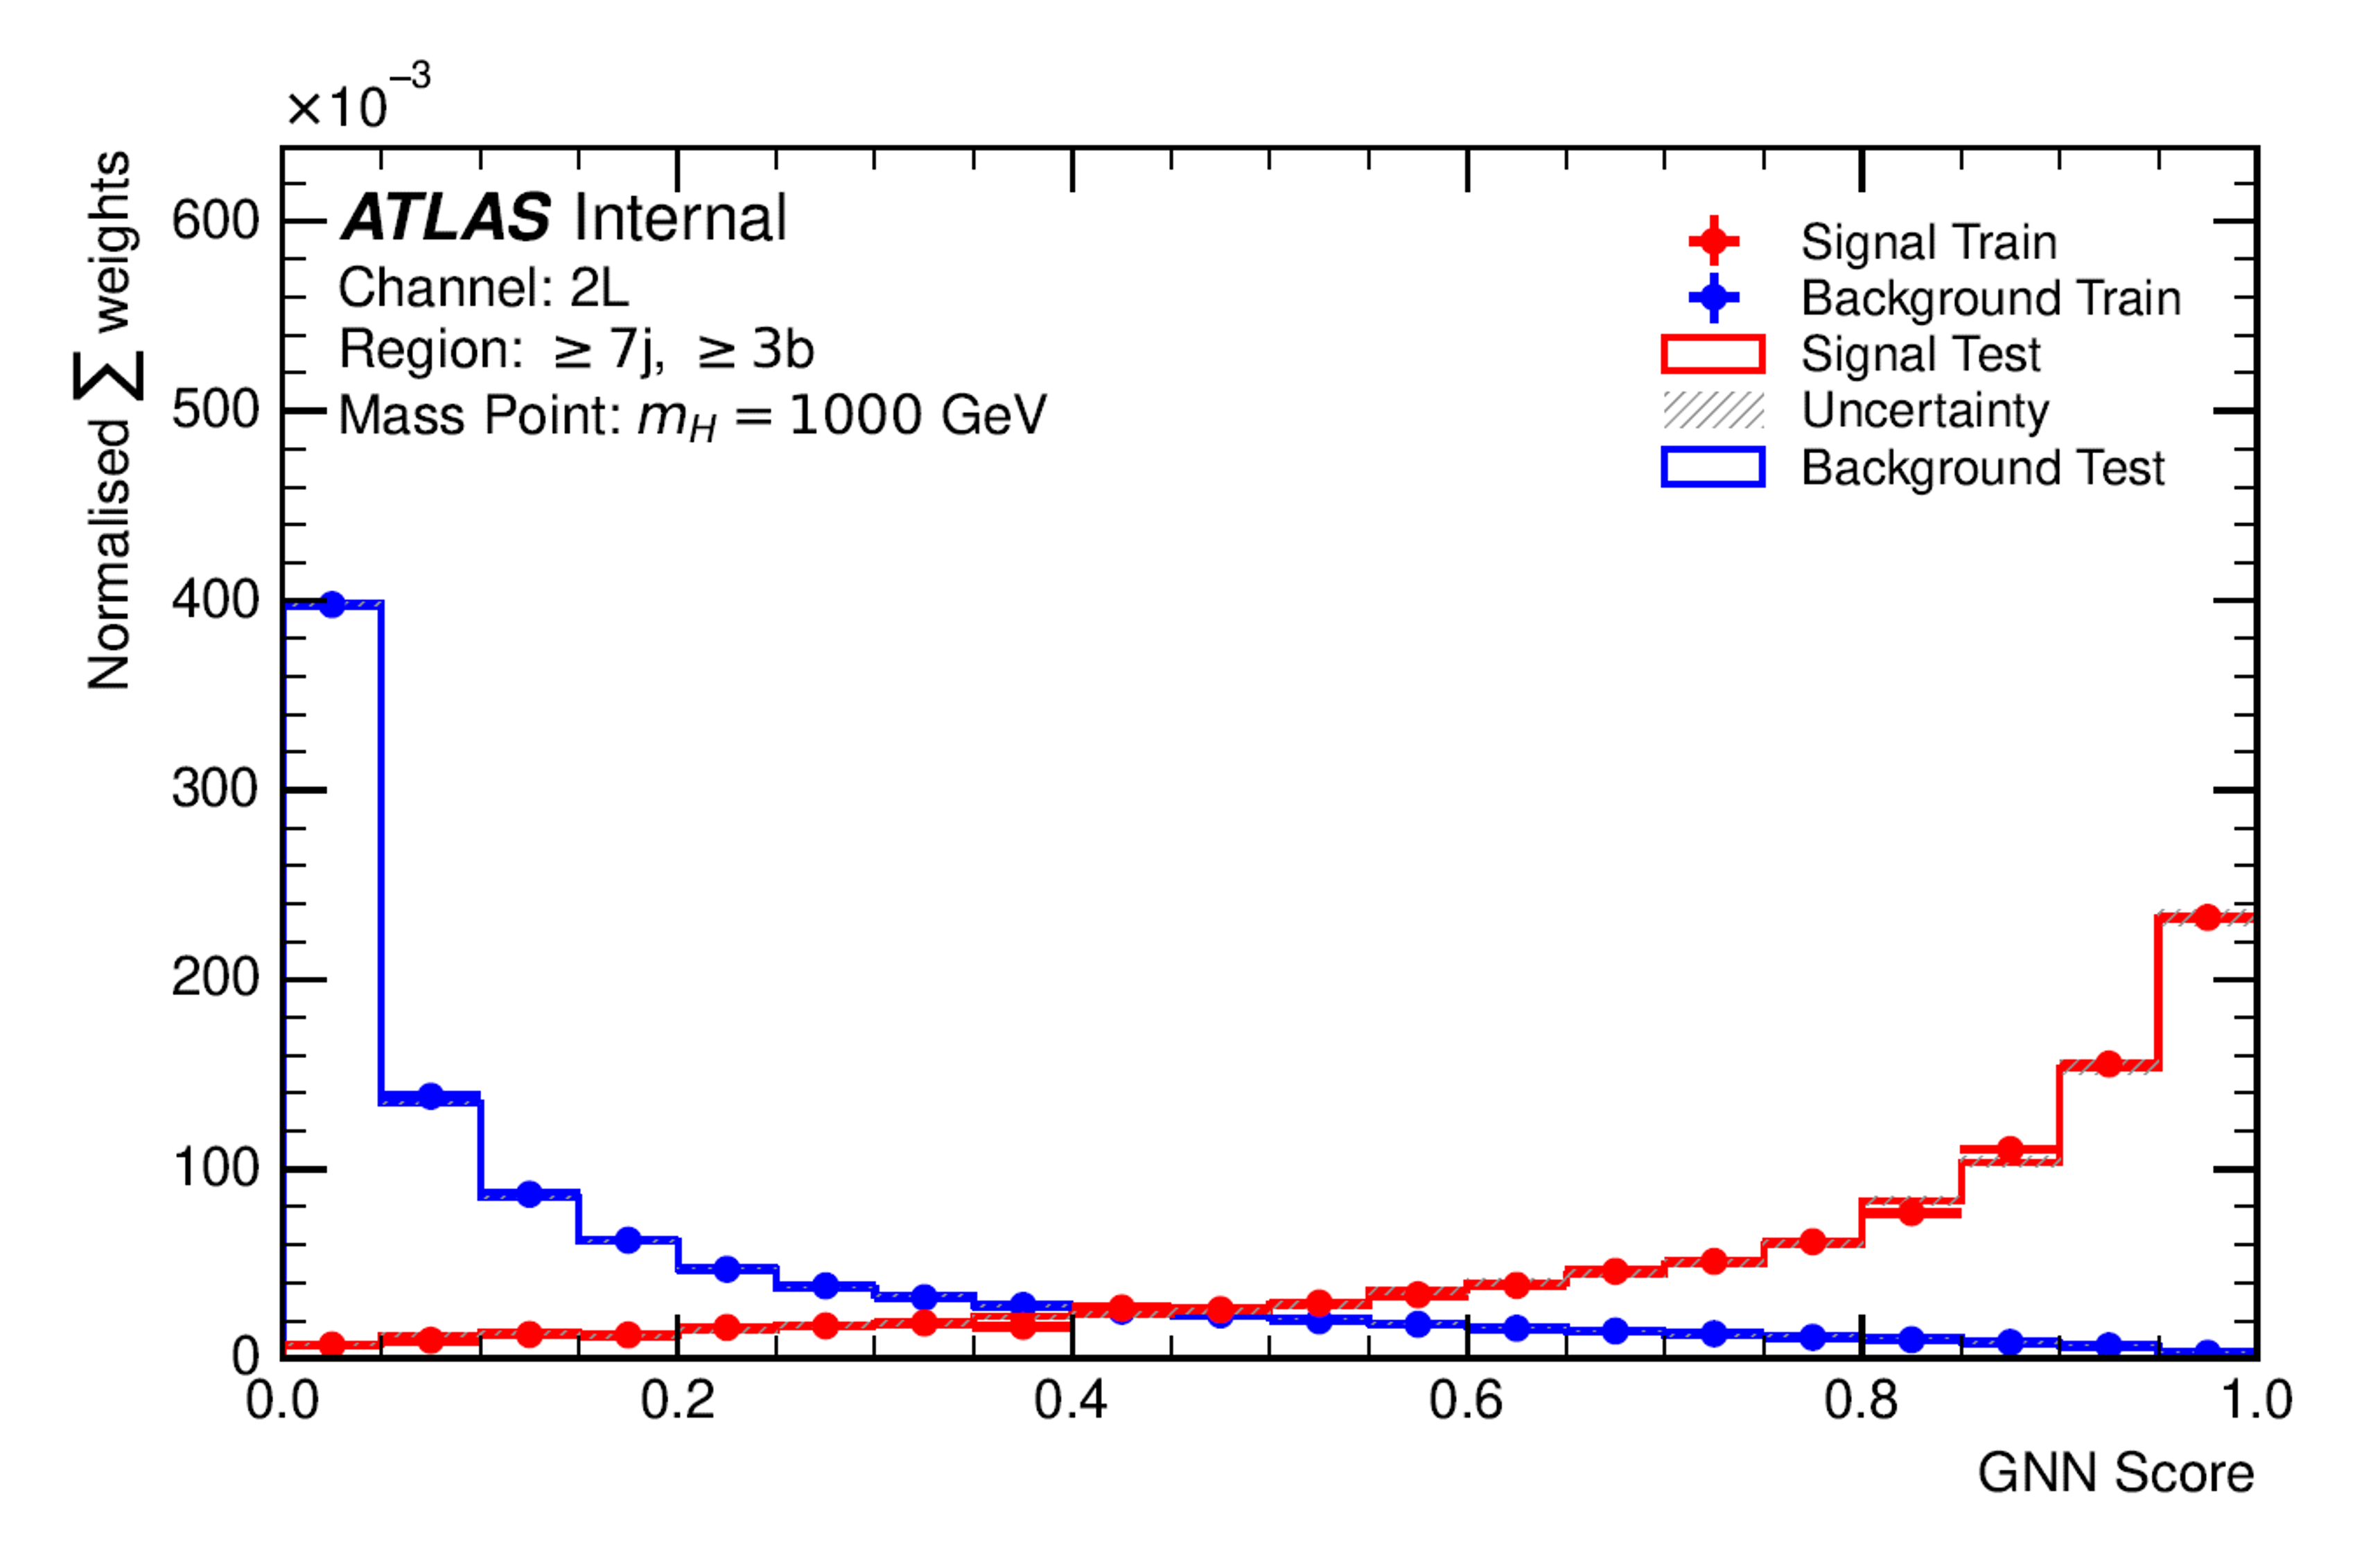
\includegraphics[width=.48\textwidth]{figures/gnn/Plots_2LOS/1000/GNN_Score_Plot_1000GeV_Inclusive.png}
        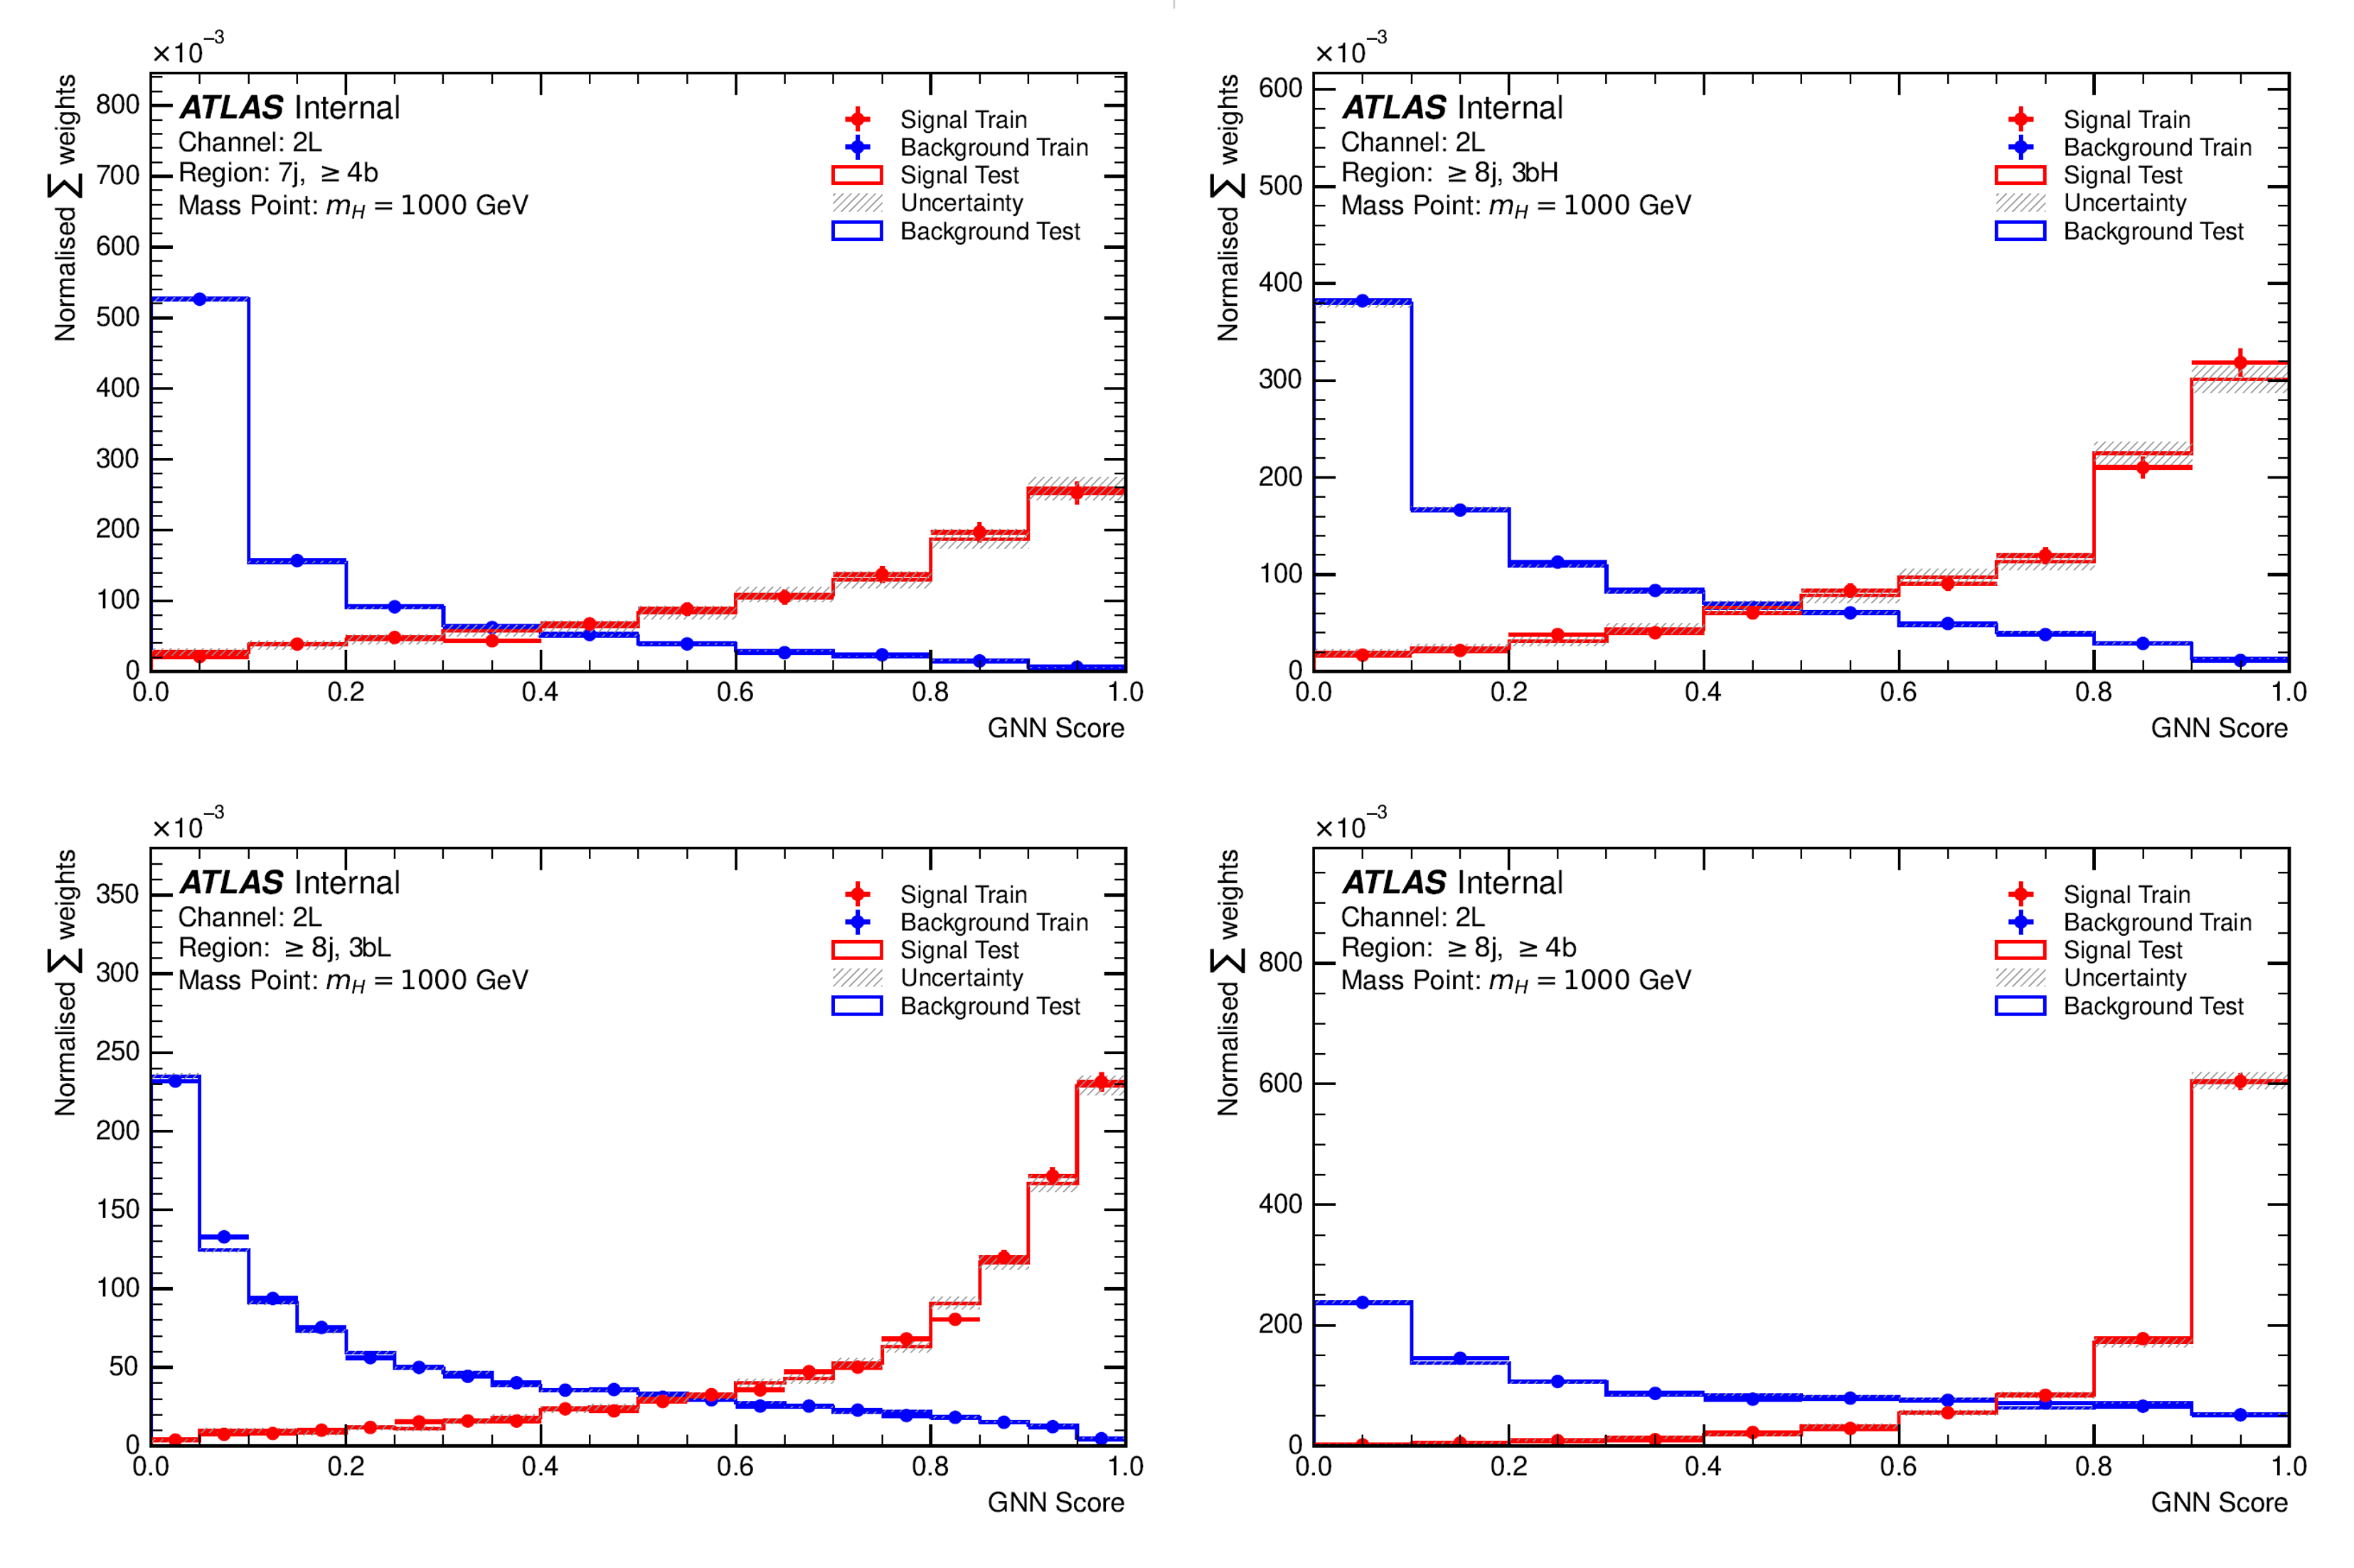
\includegraphics[width=.48\textwidth]{figures/gnn/Plots_2LOS/1000/GNN_Score_Plot_1000GeV_Split.png}
        \caption{1000 GeV mass point}
    \end{subfigure}
    \caption{Score distributions for the 2LOS GNN for several mass points. Shown in the inclusive training region (left) and four subdivided regions (right). Distributions are shown separately for models trained on even/odd event numbers and are split into training and testing results. The combined result of the cross trained model is shown in blue (signal) and red (background).}
    \label{fig:2los-gnn-scores}
\end{figure}

\begin{figure}[h!]
    \centering
    \begin{subfigure}[t]{\textwidth}
        \centering
        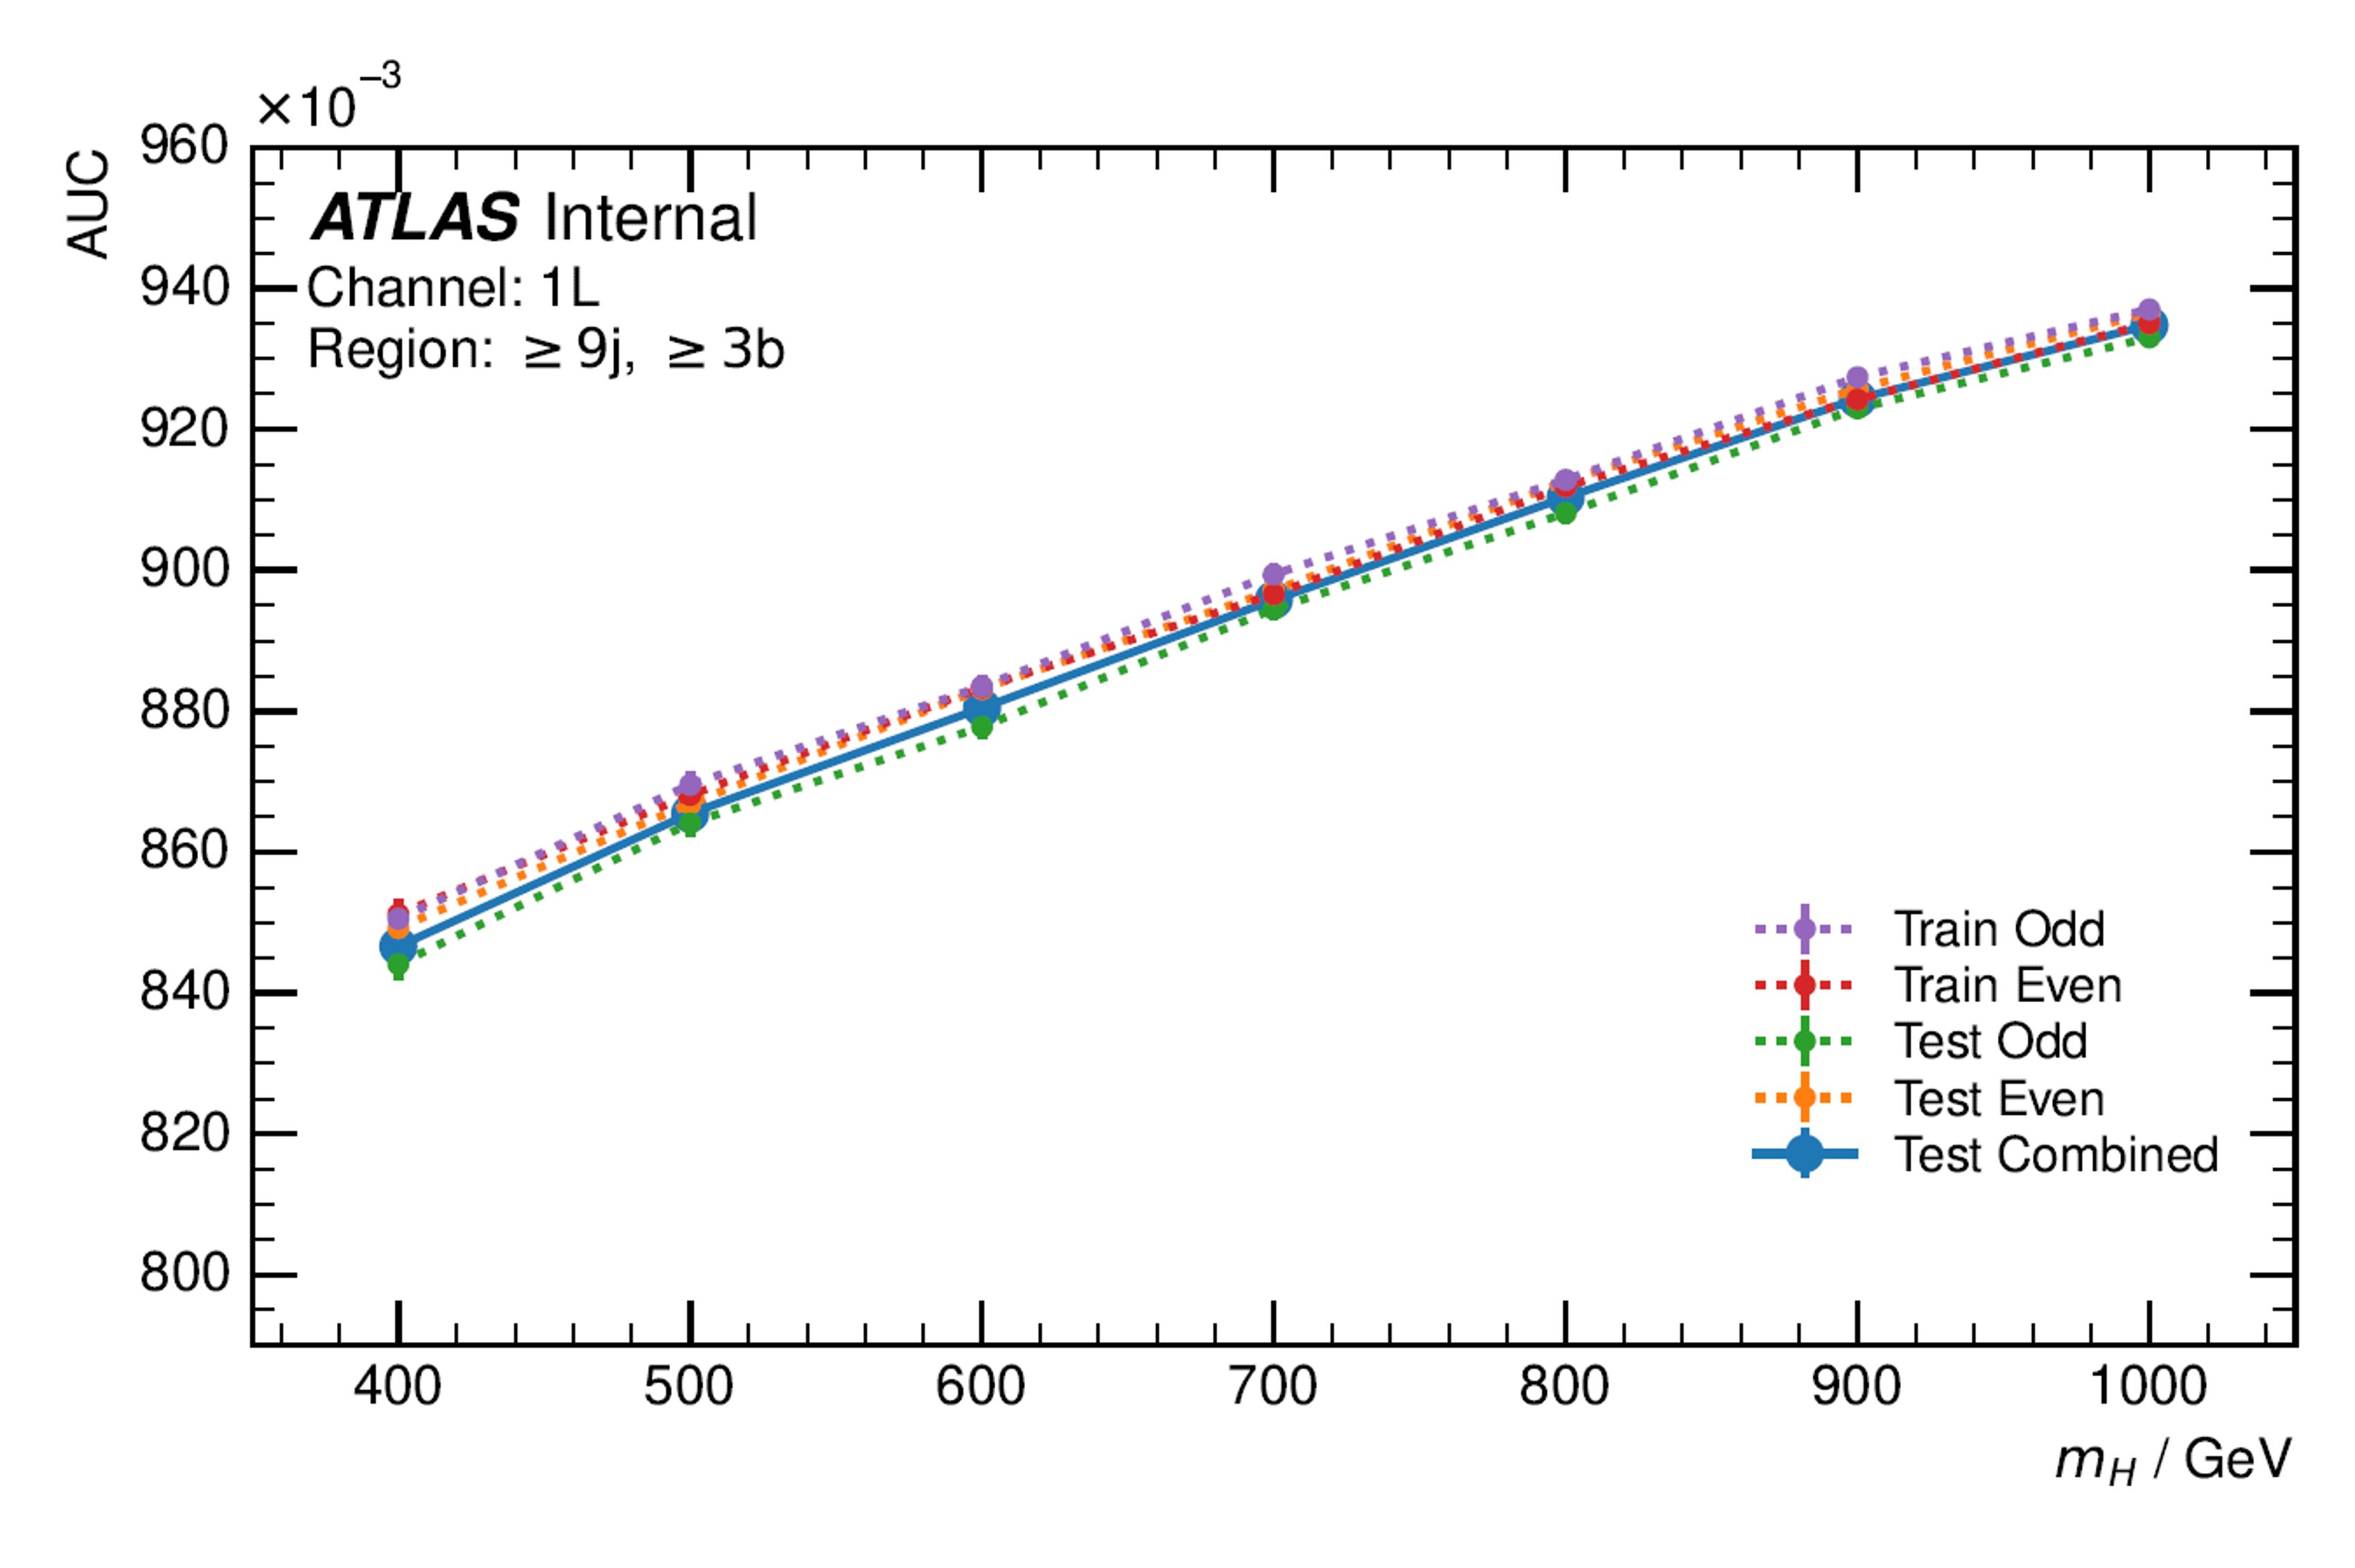
\includegraphics[width=0.48\textwidth]{figures/gnn/Plots_1L/AUC_vs_Mass_Inclusive.png}
        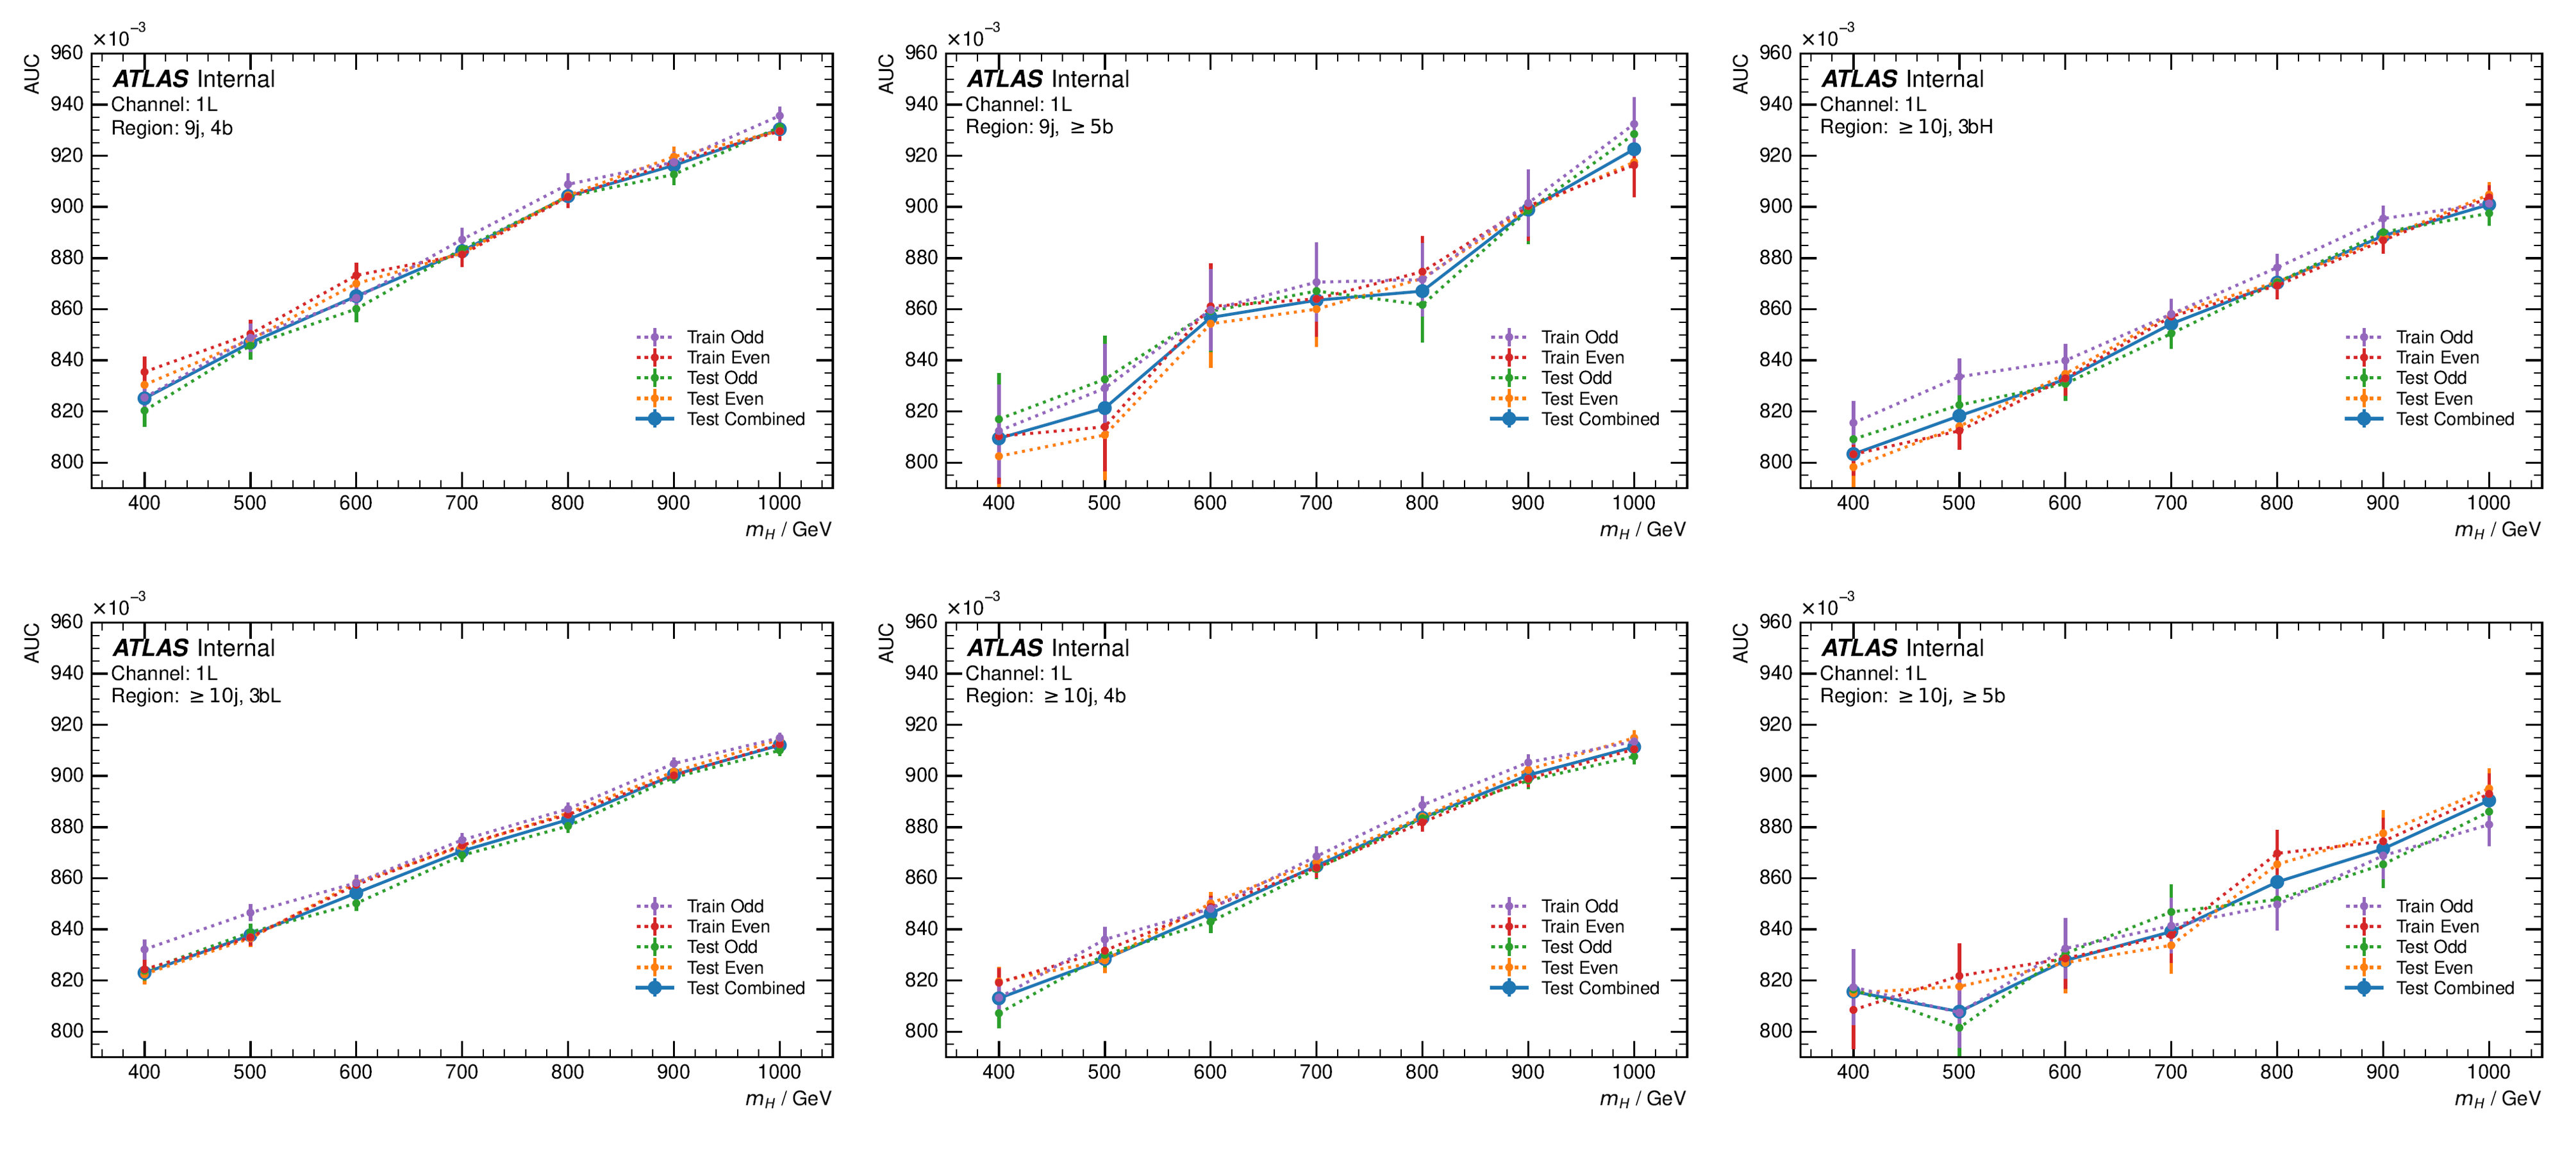
\includegraphics[width=0.48\textwidth]{figures/gnn/Plots_1L/AUC_vs_Mass_Split.png}
        \caption{1L channel}
    \end{subfigure}
    \bigskip
    \centering
    \begin{subfigure}[t]{\textwidth}
        \centering
        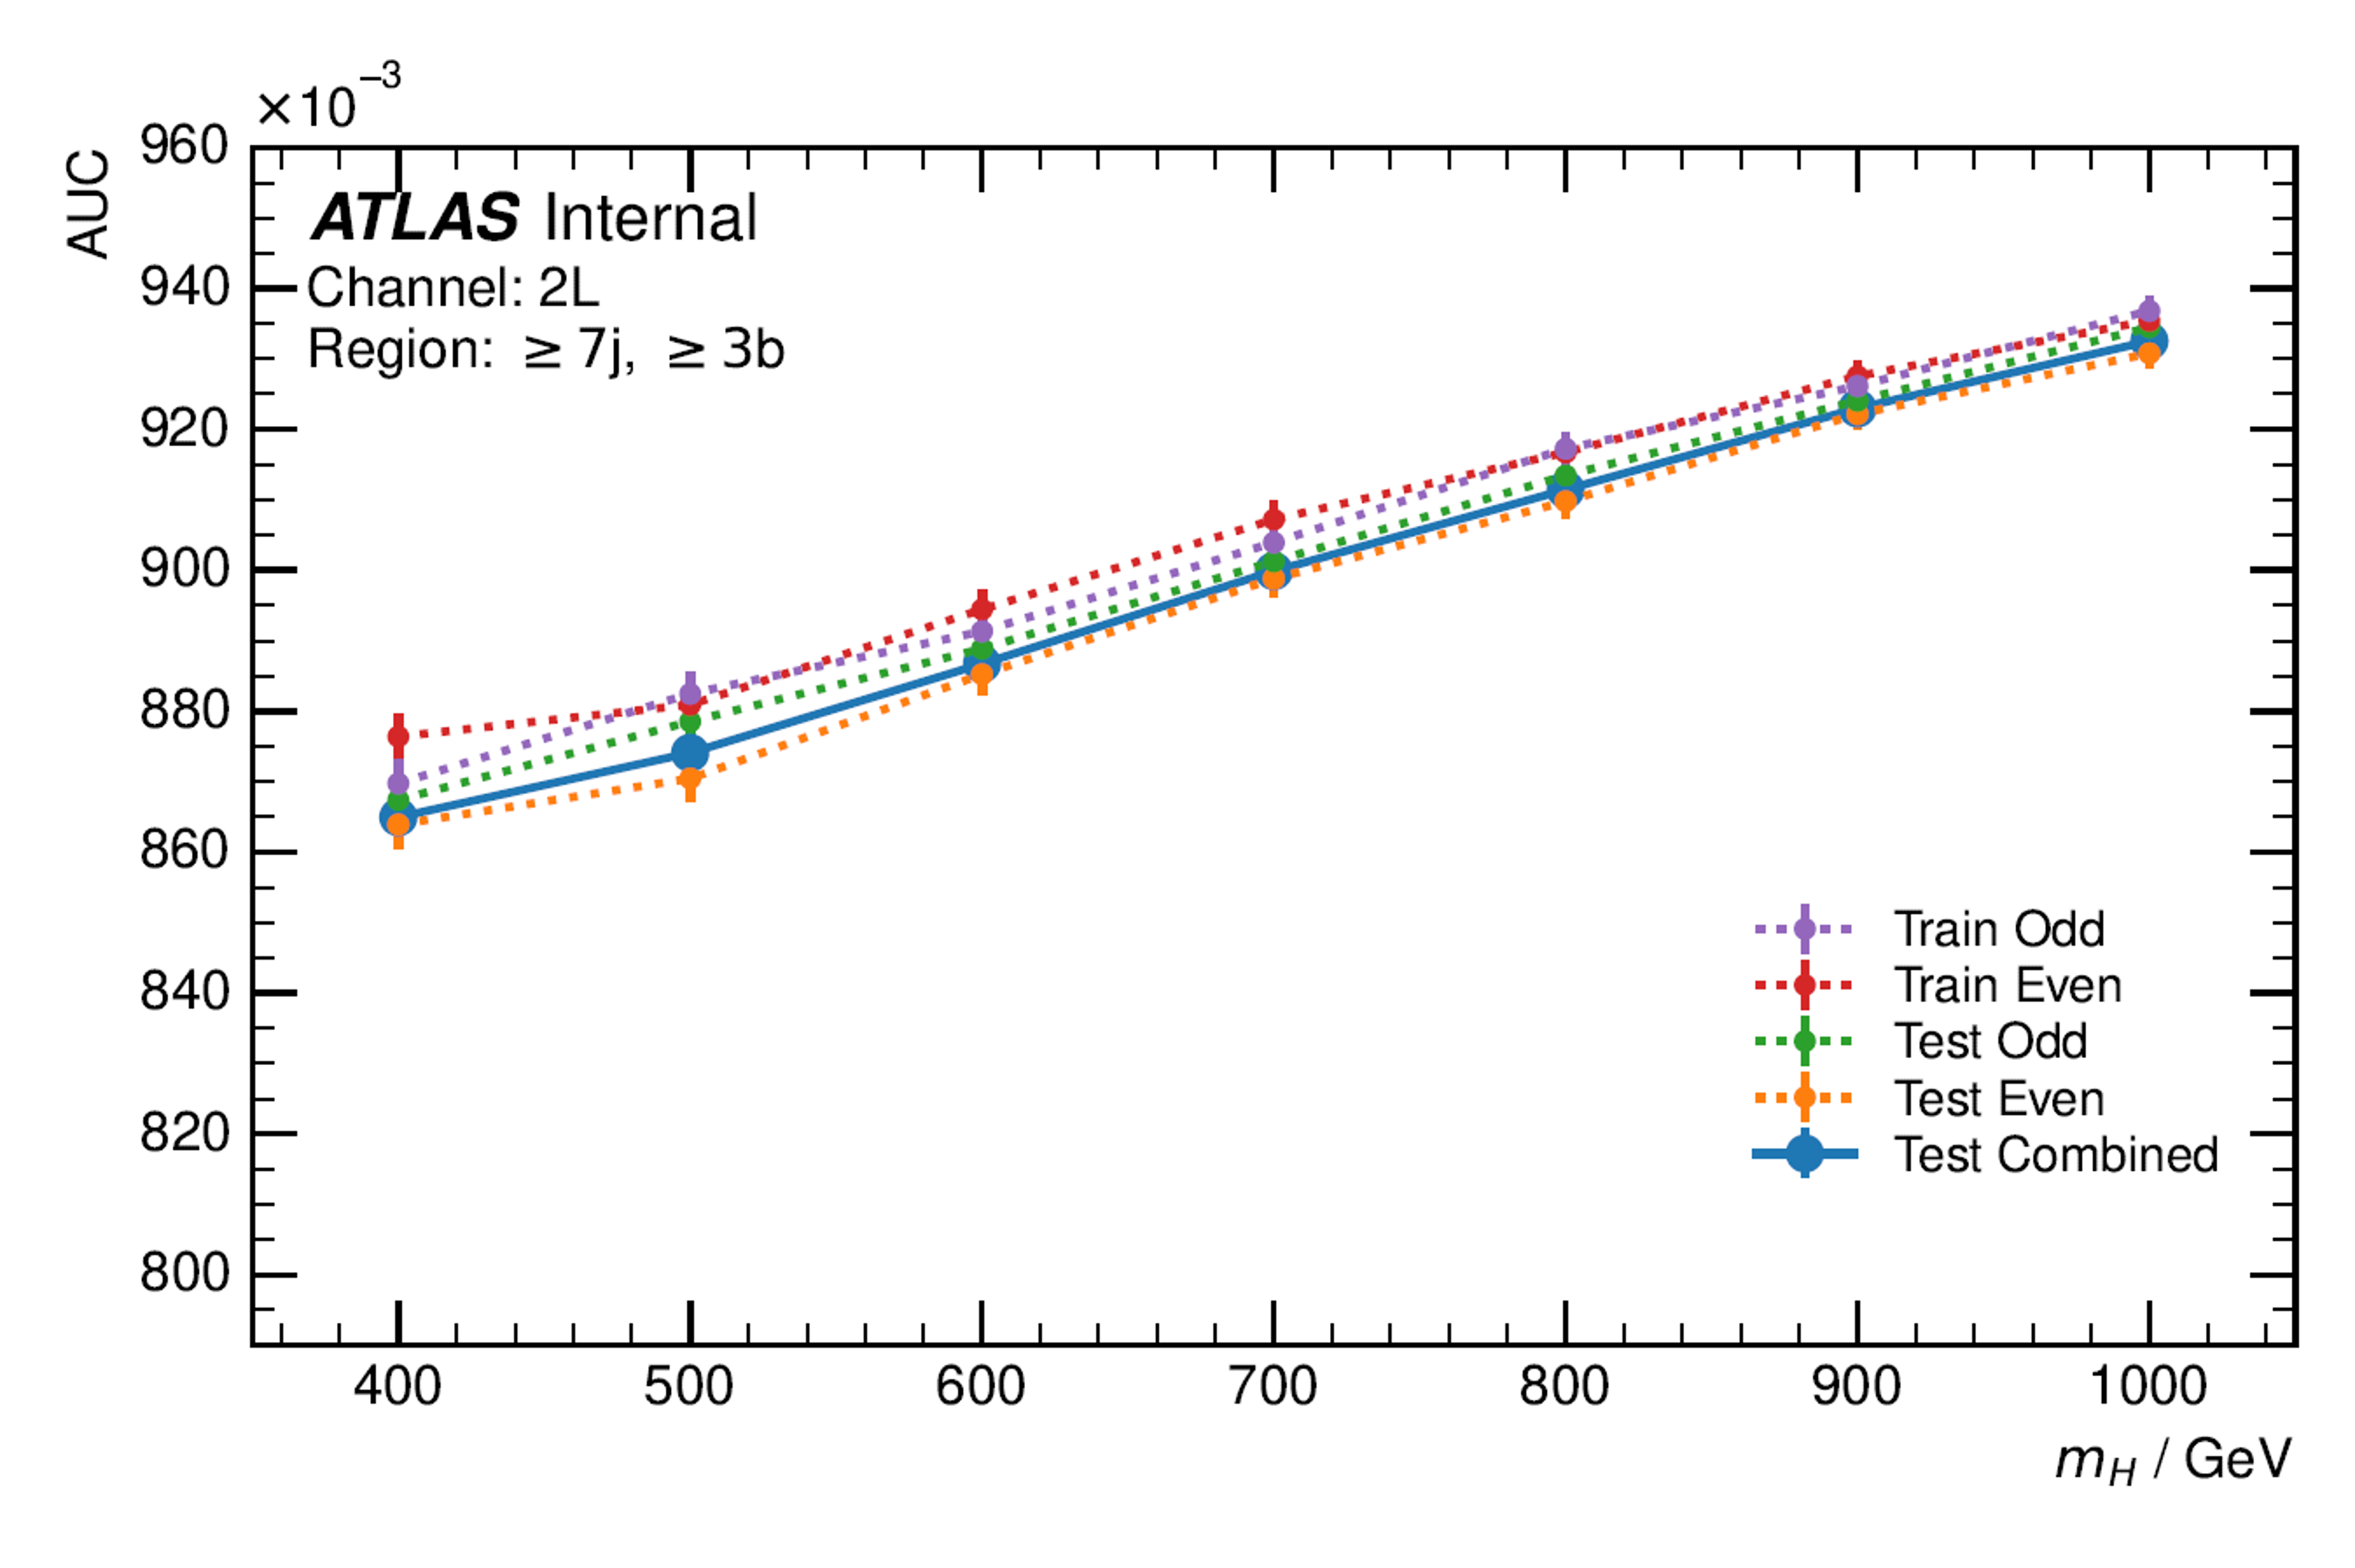
\includegraphics[width=0.48\textwidth]{figures/gnn/Plots_2LOS/AUC_vs_Mass_Inclusive.png}
        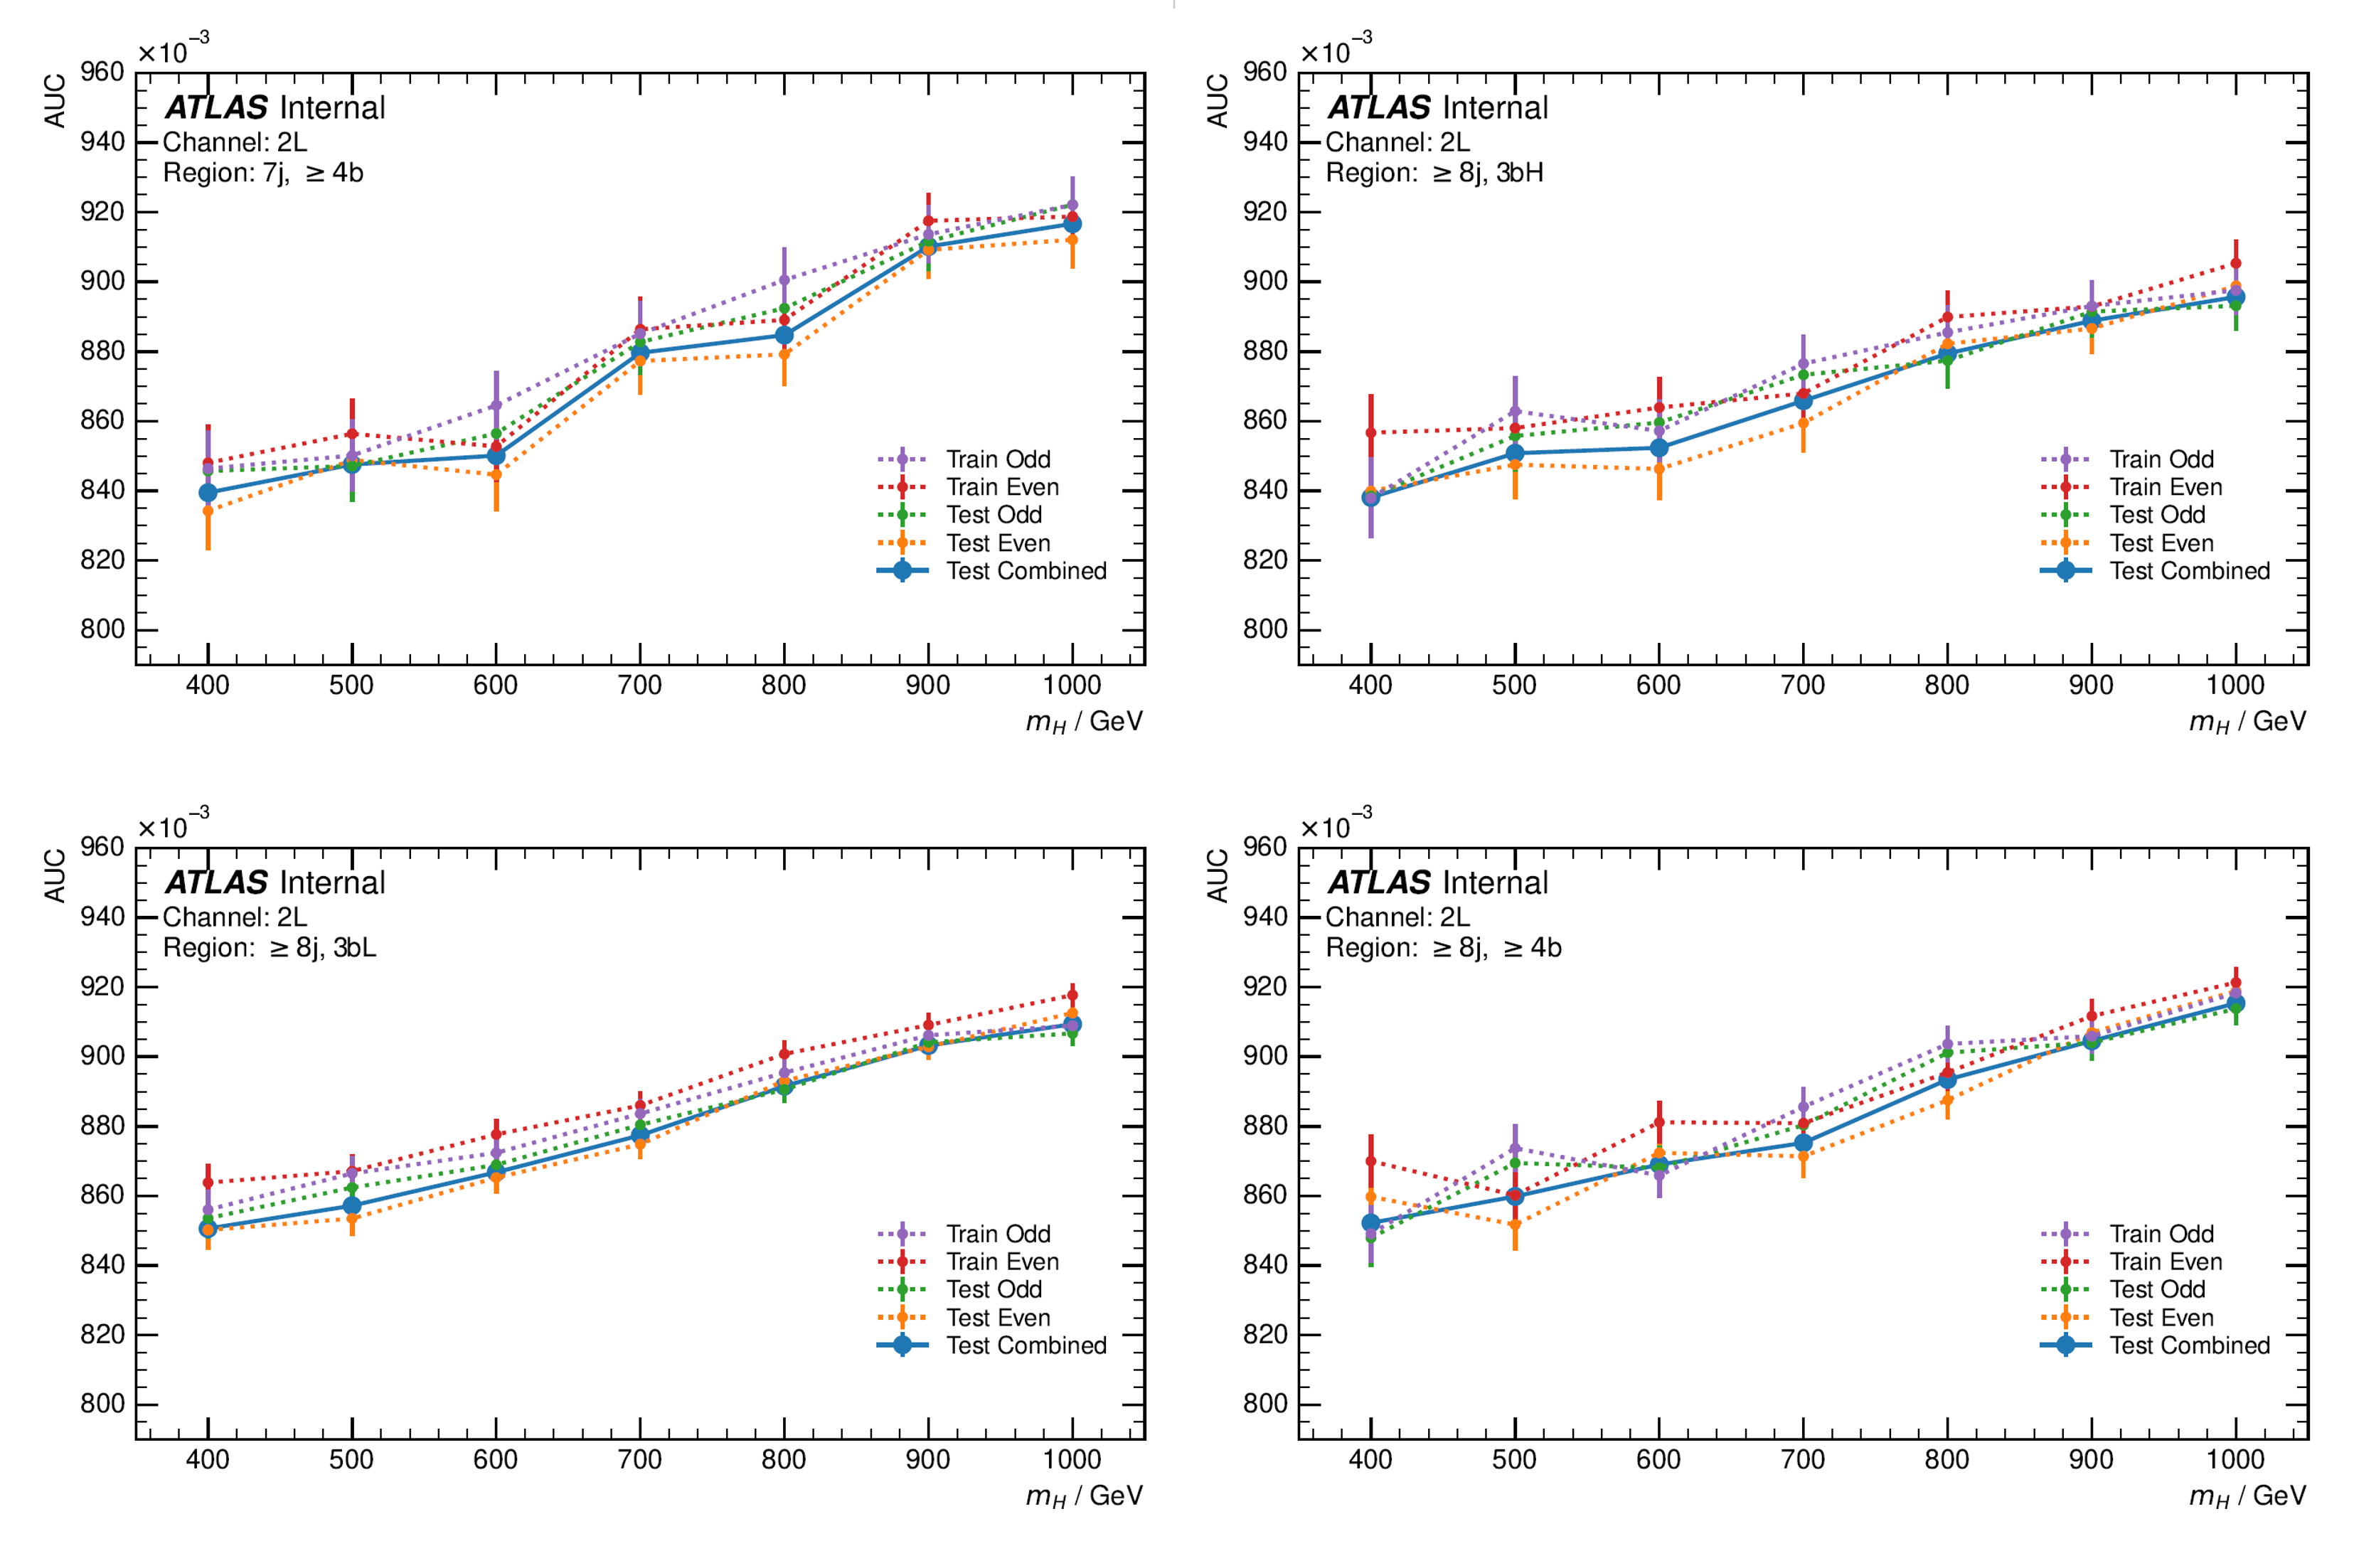
\includegraphics[width=0.48\textwidth]{figures/gnn/Plots_2LOS/AUC_vs_Mass_Split.png}
        \caption{2LOS channel}
    \end{subfigure}
    \caption{Area under ROC curves (AUC) for each mass point for 1L and 2LOS GNN models. Shown in the inclusive training region (left) and four subdivided regions (right). Separate lines are shown for training/testing results of the even/odd event trained models as well as the combined cross-trained model result.}
    \label{fig:AUCvsMass-1LOS}
\end{figure}

\begin{figure}[h!]
    \centering
    \begin{subfigure}[t]{\textwidth}
        \centering
        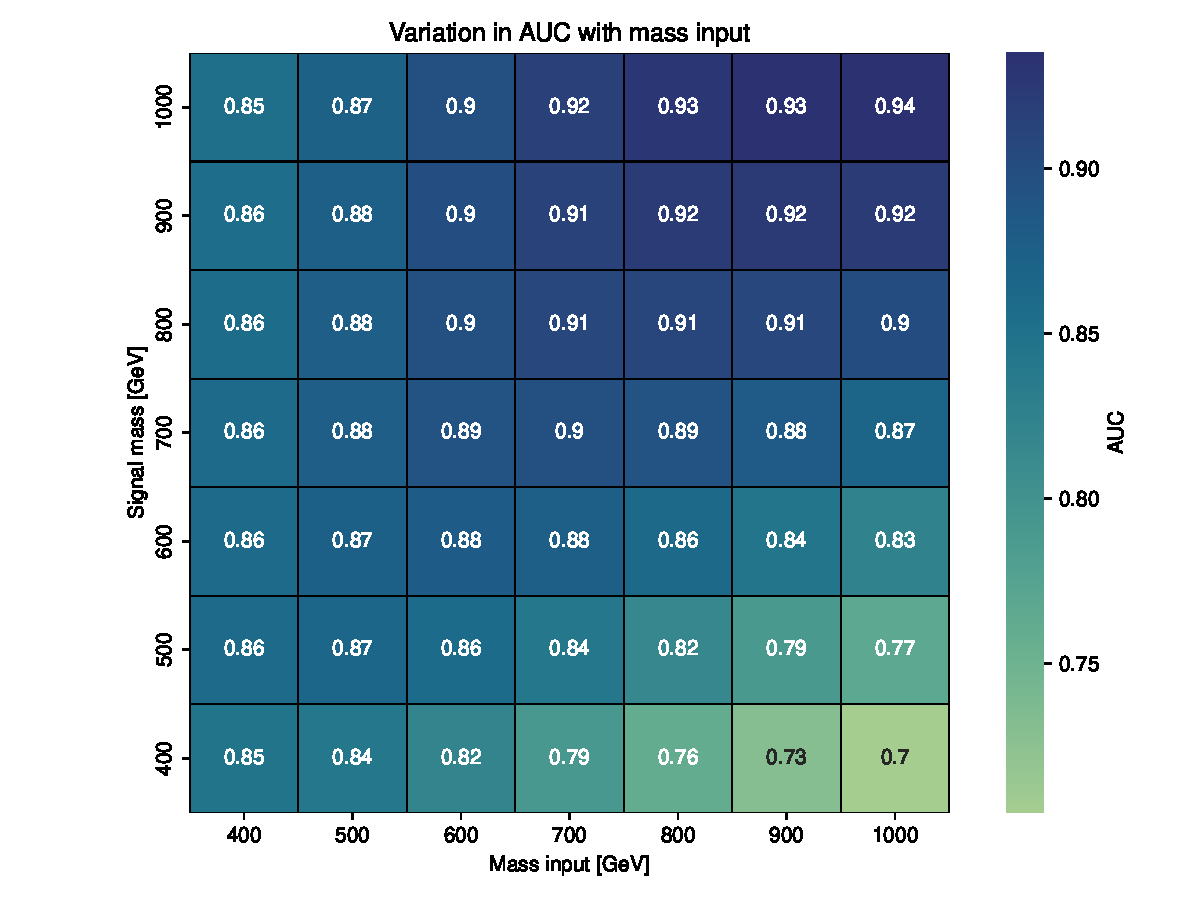
\includegraphics[height=3in]{figures/gnn/Plots_1L/AUC_mass_variations.pdf}
    \caption{1L channel}
    \end{subfigure}
    \bigskip
    \centering
    \begin{subfigure}[t]{\textwidth}
        \centering
        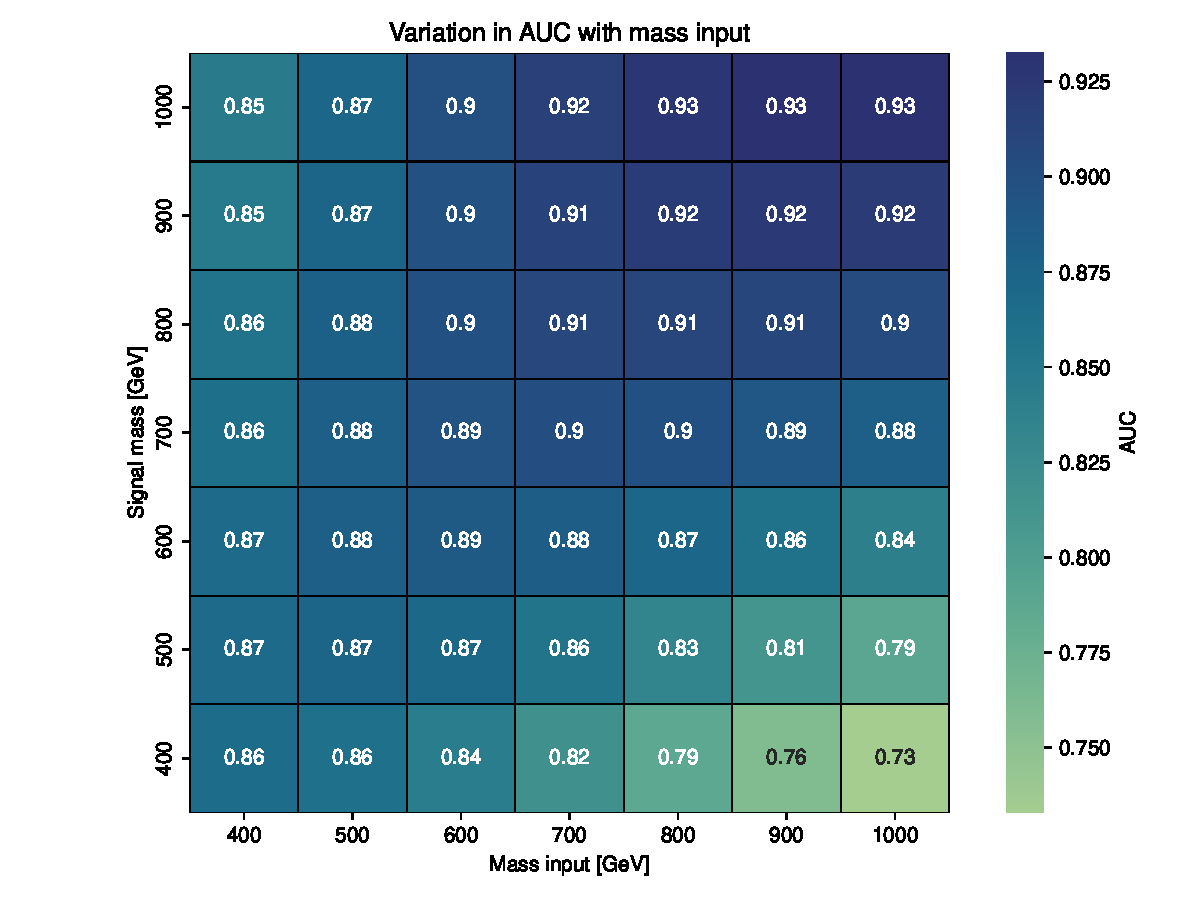
\includegraphics[height=3in]{figures/gnn/Plots_2LOS/AUC_mass_variations.pdf}
    \caption{2LOS channel}
    \end{subfigure}
    \caption{AUC as a function of pseudomass (x-axis) and various signal samples (y-axis).}
    \label{fig:gnn-AUC-mass}
\end{figure}


After training the importance of each input feature is evaluated. The importance of each feature is here defined as the change in loss when a feature in the graph is randomised. The randomisation is performed by shuffling graph features between events in the data set. The feature ranking plots are shown for both channels in figure \ref{fig:gnn-feature-ranking}. The ranking is performed using the inclusive training data set.

\begin{figure}[h!]
    \centering
    \begin{subfigure}[t]{\textwidth}
        \centering
        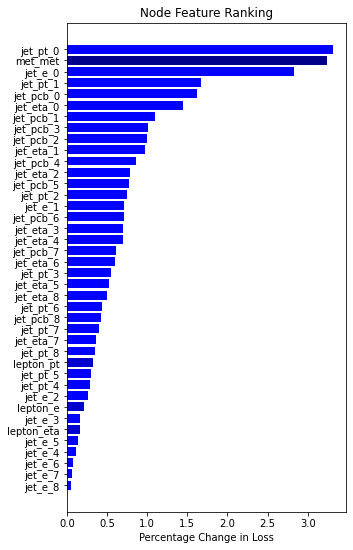
\includegraphics[height=3in]{figures/gnn/Plots_1L/NodeRanking_1L.png}
        \hskip0.3in
        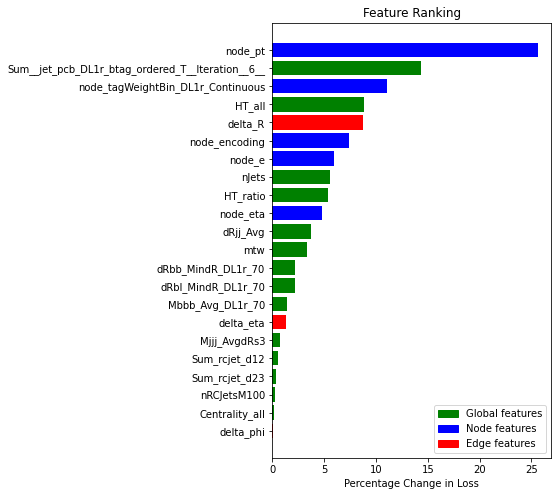
\includegraphics[height=3in]{figures/gnn/Plots_1L/FeatureRanking_1L.png}
    \caption{1L channel}
    \end{subfigure}
    \bigskip
    \centering
    \begin{subfigure}[t]{\textwidth}
        \centering
        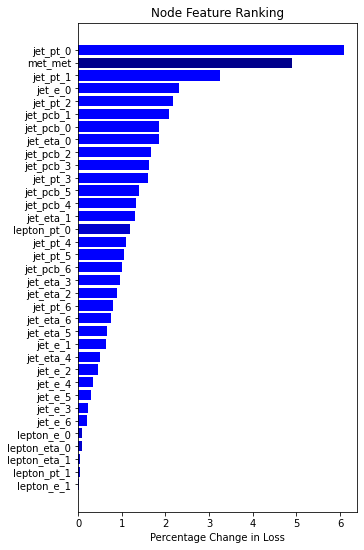
\includegraphics[height=3in]{figures/gnn/Plots_2LOS/NodeRanking_2LOS.png}
         \hskip0.3in
        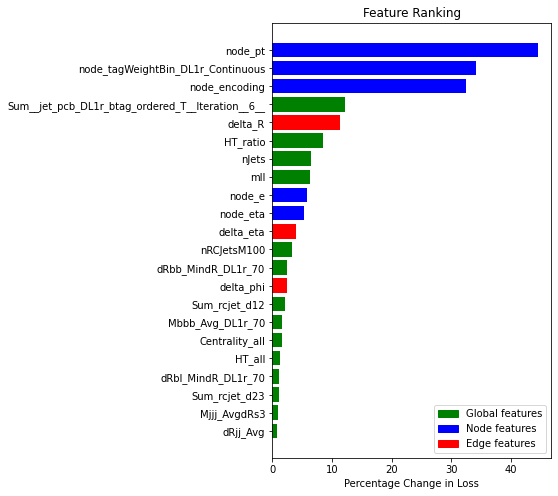
\includegraphics[height=3in]{figures/gnn/Plots_2LOS/FeatureRanking_2LOS.png}
    \caption{2LOS channel}
    \end{subfigure}
    \caption{Feature ranking of the GNN input variables. The feature ranking plot (right) includes all graph features and node/edge features are randomised inclusively of all nodes/edges in the graph. In the node feature ranking plot (left) node features are shuffled on a per object basis.}
    \label{fig:gnn-feature-ranking}
\end{figure}


